% =====================================================================================
% Sec. 5  Two sources of error (C2).  Owner: ojas.  Draft for the ACL skeleton.
%
% Every number is a macro from a committed artifact, or a design constant whose source is
% named in a comment beside it.  The skeleton's preamble inputs the two macro files (the
% paths are the skeleton's choice), e.g.
%   % Generated by scripts/figures_t9.py -- do not edit by hand.
% T9, C2 on the synthetic JSON probe.  commit 813e093c6c4972c54ec021a5d410b55df0a21a09
% Main variant ft110m-v3-visible by the pre-set rule (artifacts/probe/main_variant.json); Alt = ft110m-v3; Untuned = untuned-v3.
% Sources: artifacts/probe/results/grid_<tag>.json, rho_check_<tag>.json, val_rescored.json, history_<tag>.jsonl.
%
% Grid cells: \CTwo[Alt|Untuned]<Rule><Q>at<Rho><K>[Lo|Hi], e.g. \CTwoConfAatRhoOneKEight
%   no variant word = the main variant; Rule: Conf = confidence top-k, Rand = random positions
%   Q: A = (A) dependency, B = (B) estimation, nats per field (mean over the instances at that rho);
%      ShareA = (A) as a percentage of (A)+(B)
%   Rho: RhoZero, RhoQuarter, RhoHalf, RhoThreeQuarters, RhoOne;  K: KOne, KTwo, KFour, KEight
%   Lo/Hi (main variant only): 95% bootstrap interval, instances resampled
% Crossover: \CTwo[Alt|Untuned]<Rule>CrossKat<Rho> = the first k at which mean (A) > mean (B);
%   ...CrossKCIat<Rho> = the first k at which the 95% interval of (A)-(B) is above 0;
%   -- = at no k <= 8.  ...CrossRhoMin = the smallest rho with a crossover, ...ShareAMax = the largest ShareA.
%
% ft110m-v3-visible (main variant): 1000 instances, 10000 resamples
\newcommand{\CTwoConfAatRhoZeroKOne}{0.000}
\newcommand{\CTwoConfAatRhoZeroKOneLo}{0.000}
\newcommand{\CTwoConfAatRhoZeroKOneHi}{0.000}
\newcommand{\CTwoConfBatRhoZeroKOne}{0.032}
\newcommand{\CTwoConfBatRhoZeroKOneLo}{0.030}
\newcommand{\CTwoConfBatRhoZeroKOneHi}{0.035}
\newcommand{\CTwoConfShareAatRhoZeroKOne}{0}
\newcommand{\CTwoConfAatRhoZeroKTwo}{0.000}
\newcommand{\CTwoConfAatRhoZeroKTwoLo}{0.000}
\newcommand{\CTwoConfAatRhoZeroKTwoHi}{0.000}
\newcommand{\CTwoConfBatRhoZeroKTwo}{0.032}
\newcommand{\CTwoConfBatRhoZeroKTwoLo}{0.029}
\newcommand{\CTwoConfBatRhoZeroKTwoHi}{0.034}
\newcommand{\CTwoConfShareAatRhoZeroKTwo}{0}
\newcommand{\CTwoConfAatRhoZeroKFour}{0.000}
\newcommand{\CTwoConfAatRhoZeroKFourLo}{0.000}
\newcommand{\CTwoConfAatRhoZeroKFourHi}{0.000}
\newcommand{\CTwoConfBatRhoZeroKFour}{0.031}
\newcommand{\CTwoConfBatRhoZeroKFourLo}{0.029}
\newcommand{\CTwoConfBatRhoZeroKFourHi}{0.033}
\newcommand{\CTwoConfShareAatRhoZeroKFour}{0}
\newcommand{\CTwoConfAatRhoZeroKEight}{0.000}
\newcommand{\CTwoConfAatRhoZeroKEightLo}{0.000}
\newcommand{\CTwoConfAatRhoZeroKEightHi}{0.000}
\newcommand{\CTwoConfBatRhoZeroKEight}{0.029}
\newcommand{\CTwoConfBatRhoZeroKEightLo}{0.027}
\newcommand{\CTwoConfBatRhoZeroKEightHi}{0.031}
\newcommand{\CTwoConfShareAatRhoZeroKEight}{0}
\newcommand{\CTwoConfAatRhoQuarterKOne}{0.000}
\newcommand{\CTwoConfAatRhoQuarterKOneLo}{0.000}
\newcommand{\CTwoConfAatRhoQuarterKOneHi}{0.000}
\newcommand{\CTwoConfBatRhoQuarterKOne}{0.060}
\newcommand{\CTwoConfBatRhoQuarterKOneLo}{0.055}
\newcommand{\CTwoConfBatRhoQuarterKOneHi}{0.066}
\newcommand{\CTwoConfShareAatRhoQuarterKOne}{0}
\newcommand{\CTwoConfAatRhoQuarterKTwo}{0.004}
\newcommand{\CTwoConfAatRhoQuarterKTwoLo}{0.003}
\newcommand{\CTwoConfAatRhoQuarterKTwoHi}{0.005}
\newcommand{\CTwoConfBatRhoQuarterKTwo}{0.056}
\newcommand{\CTwoConfBatRhoQuarterKTwoLo}{0.051}
\newcommand{\CTwoConfBatRhoQuarterKTwoHi}{0.061}
\newcommand{\CTwoConfShareAatRhoQuarterKTwo}{7}
\newcommand{\CTwoConfAatRhoQuarterKFour}{0.011}
\newcommand{\CTwoConfAatRhoQuarterKFourLo}{0.010}
\newcommand{\CTwoConfAatRhoQuarterKFourHi}{0.013}
\newcommand{\CTwoConfBatRhoQuarterKFour}{0.049}
\newcommand{\CTwoConfBatRhoQuarterKFourLo}{0.045}
\newcommand{\CTwoConfBatRhoQuarterKFourHi}{0.054}
\newcommand{\CTwoConfShareAatRhoQuarterKFour}{19}
\newcommand{\CTwoConfAatRhoQuarterKEight}{0.025}
\newcommand{\CTwoConfAatRhoQuarterKEightLo}{0.022}
\newcommand{\CTwoConfAatRhoQuarterKEightHi}{0.027}
\newcommand{\CTwoConfBatRhoQuarterKEight}{0.037}
\newcommand{\CTwoConfBatRhoQuarterKEightLo}{0.034}
\newcommand{\CTwoConfBatRhoQuarterKEightHi}{0.041}
\newcommand{\CTwoConfShareAatRhoQuarterKEight}{40}
\newcommand{\CTwoConfAatRhoHalfKOne}{0.000}
\newcommand{\CTwoConfAatRhoHalfKOneLo}{0.000}
\newcommand{\CTwoConfAatRhoHalfKOneHi}{0.000}
\newcommand{\CTwoConfBatRhoHalfKOne}{0.118}
\newcommand{\CTwoConfBatRhoHalfKOneLo}{0.109}
\newcommand{\CTwoConfBatRhoHalfKOneHi}{0.127}
\newcommand{\CTwoConfShareAatRhoHalfKOne}{0}
\newcommand{\CTwoConfAatRhoHalfKTwo}{0.016}
\newcommand{\CTwoConfAatRhoHalfKTwoLo}{0.012}
\newcommand{\CTwoConfAatRhoHalfKTwoHi}{0.019}
\newcommand{\CTwoConfBatRhoHalfKTwo}{0.105}
\newcommand{\CTwoConfBatRhoHalfKTwoLo}{0.096}
\newcommand{\CTwoConfBatRhoHalfKTwoHi}{0.113}
\newcommand{\CTwoConfShareAatRhoHalfKTwo}{13}
\newcommand{\CTwoConfAatRhoHalfKFour}{0.037}
\newcommand{\CTwoConfAatRhoHalfKFourLo}{0.033}
\newcommand{\CTwoConfAatRhoHalfKFourHi}{0.041}
\newcommand{\CTwoConfBatRhoHalfKFour}{0.088}
\newcommand{\CTwoConfBatRhoHalfKFourLo}{0.080}
\newcommand{\CTwoConfBatRhoHalfKFourHi}{0.096}
\newcommand{\CTwoConfShareAatRhoHalfKFour}{30}
\newcommand{\CTwoConfAatRhoHalfKEight}{0.078}
\newcommand{\CTwoConfAatRhoHalfKEightLo}{0.072}
\newcommand{\CTwoConfAatRhoHalfKEightHi}{0.084}
\newcommand{\CTwoConfBatRhoHalfKEight}{0.056}
\newcommand{\CTwoConfBatRhoHalfKEightLo}{0.050}
\newcommand{\CTwoConfBatRhoHalfKEightHi}{0.062}
\newcommand{\CTwoConfShareAatRhoHalfKEight}{58}
\newcommand{\CTwoConfAatRhoThreeQuartersKOne}{0.000}
\newcommand{\CTwoConfAatRhoThreeQuartersKOneLo}{0.000}
\newcommand{\CTwoConfAatRhoThreeQuartersKOneHi}{0.000}
\newcommand{\CTwoConfBatRhoThreeQuartersKOne}{0.217}
\newcommand{\CTwoConfBatRhoThreeQuartersKOneLo}{0.202}
\newcommand{\CTwoConfBatRhoThreeQuartersKOneHi}{0.232}
\newcommand{\CTwoConfShareAatRhoThreeQuartersKOne}{0}
\newcommand{\CTwoConfAatRhoThreeQuartersKTwo}{0.049}
\newcommand{\CTwoConfAatRhoThreeQuartersKTwoLo}{0.041}
\newcommand{\CTwoConfAatRhoThreeQuartersKTwoHi}{0.058}
\newcommand{\CTwoConfBatRhoThreeQuartersKTwo}{0.170}
\newcommand{\CTwoConfBatRhoThreeQuartersKTwoLo}{0.156}
\newcommand{\CTwoConfBatRhoThreeQuartersKTwoHi}{0.184}
\newcommand{\CTwoConfShareAatRhoThreeQuartersKTwo}{22}
\newcommand{\CTwoConfAatRhoThreeQuartersKFour}{0.107}
\newcommand{\CTwoConfAatRhoThreeQuartersKFourLo}{0.096}
\newcommand{\CTwoConfAatRhoThreeQuartersKFourHi}{0.119}
\newcommand{\CTwoConfBatRhoThreeQuartersKFour}{0.120}
\newcommand{\CTwoConfBatRhoThreeQuartersKFourLo}{0.108}
\newcommand{\CTwoConfBatRhoThreeQuartersKFourHi}{0.132}
\newcommand{\CTwoConfShareAatRhoThreeQuartersKFour}{47}
\newcommand{\CTwoConfAatRhoThreeQuartersKEight}{0.177}
\newcommand{\CTwoConfAatRhoThreeQuartersKEightLo}{0.166}
\newcommand{\CTwoConfAatRhoThreeQuartersKEightHi}{0.188}
\newcommand{\CTwoConfBatRhoThreeQuartersKEight}{0.064}
\newcommand{\CTwoConfBatRhoThreeQuartersKEightLo}{0.056}
\newcommand{\CTwoConfBatRhoThreeQuartersKEightHi}{0.071}
\newcommand{\CTwoConfShareAatRhoThreeQuartersKEight}{74}
\newcommand{\CTwoConfAatRhoOneKOne}{0.000}
\newcommand{\CTwoConfAatRhoOneKOneLo}{0.000}
\newcommand{\CTwoConfAatRhoOneKOneHi}{0.000}
\newcommand{\CTwoConfBatRhoOneKOne}{0.411}
\newcommand{\CTwoConfBatRhoOneKOneLo}{0.384}
\newcommand{\CTwoConfBatRhoOneKOneHi}{0.439}
\newcommand{\CTwoConfShareAatRhoOneKOne}{0}
\newcommand{\CTwoConfAatRhoOneKTwo}{0.124}
\newcommand{\CTwoConfAatRhoOneKTwoLo}{0.108}
\newcommand{\CTwoConfAatRhoOneKTwoHi}{0.140}
\newcommand{\CTwoConfBatRhoOneKTwo}{0.289}
\newcommand{\CTwoConfBatRhoOneKTwoLo}{0.265}
\newcommand{\CTwoConfBatRhoOneKTwoHi}{0.314}
\newcommand{\CTwoConfShareAatRhoOneKTwo}{30}
\newcommand{\CTwoConfAatRhoOneKFour}{0.234}
\newcommand{\CTwoConfAatRhoOneKFourLo}{0.216}
\newcommand{\CTwoConfAatRhoOneKFourHi}{0.254}
\newcommand{\CTwoConfBatRhoOneKFour}{0.193}
\newcommand{\CTwoConfBatRhoOneKFourLo}{0.172}
\newcommand{\CTwoConfBatRhoOneKFourHi}{0.215}
\newcommand{\CTwoConfShareAatRhoOneKFour}{55}
\newcommand{\CTwoConfAatRhoOneKEight}{0.338}
\newcommand{\CTwoConfAatRhoOneKEightLo}{0.320}
\newcommand{\CTwoConfAatRhoOneKEightHi}{0.355}
\newcommand{\CTwoConfBatRhoOneKEight}{0.109}
\newcommand{\CTwoConfBatRhoOneKEightLo}{0.095}
\newcommand{\CTwoConfBatRhoOneKEightHi}{0.123}
\newcommand{\CTwoConfShareAatRhoOneKEight}{76}
\newcommand{\CTwoConfCrossKatRhoZero}{--}
\newcommand{\CTwoConfCrossKCIatRhoZero}{--}
\newcommand{\CTwoConfCrossKatRhoQuarter}{--}
\newcommand{\CTwoConfCrossKCIatRhoQuarter}{--}
\newcommand{\CTwoConfCrossKatRhoHalf}{8}
\newcommand{\CTwoConfCrossKCIatRhoHalf}{8}
\newcommand{\CTwoConfCrossKatRhoThreeQuarters}{8}
\newcommand{\CTwoConfCrossKCIatRhoThreeQuarters}{8}
\newcommand{\CTwoConfCrossKatRhoOne}{4}
\newcommand{\CTwoConfCrossKCIatRhoOne}{4}
\newcommand{\CTwoConfCrossRhoMin}{0.5}
\newcommand{\CTwoConfShareAMax}{76}
\newcommand{\CTwoRandAatRhoZeroKOne}{0.000}
\newcommand{\CTwoRandAatRhoZeroKOneLo}{0.000}
\newcommand{\CTwoRandAatRhoZeroKOneHi}{0.000}
\newcommand{\CTwoRandBatRhoZeroKOne}{0.032}
\newcommand{\CTwoRandBatRhoZeroKOneLo}{0.030}
\newcommand{\CTwoRandBatRhoZeroKOneHi}{0.035}
\newcommand{\CTwoRandShareAatRhoZeroKOne}{0}
\newcommand{\CTwoRandAatRhoZeroKTwo}{0.000}
\newcommand{\CTwoRandAatRhoZeroKTwoLo}{0.000}
\newcommand{\CTwoRandAatRhoZeroKTwoHi}{0.000}
\newcommand{\CTwoRandBatRhoZeroKTwo}{0.032}
\newcommand{\CTwoRandBatRhoZeroKTwoLo}{0.029}
\newcommand{\CTwoRandBatRhoZeroKTwoHi}{0.035}
\newcommand{\CTwoRandShareAatRhoZeroKTwo}{0}
\newcommand{\CTwoRandAatRhoZeroKFour}{0.000}
\newcommand{\CTwoRandAatRhoZeroKFourLo}{0.000}
\newcommand{\CTwoRandAatRhoZeroKFourHi}{0.000}
\newcommand{\CTwoRandBatRhoZeroKFour}{0.030}
\newcommand{\CTwoRandBatRhoZeroKFourLo}{0.028}
\newcommand{\CTwoRandBatRhoZeroKFourHi}{0.033}
\newcommand{\CTwoRandShareAatRhoZeroKFour}{0}
\newcommand{\CTwoRandAatRhoZeroKEight}{0.000}
\newcommand{\CTwoRandAatRhoZeroKEightLo}{0.000}
\newcommand{\CTwoRandAatRhoZeroKEightHi}{0.000}
\newcommand{\CTwoRandBatRhoZeroKEight}{0.029}
\newcommand{\CTwoRandBatRhoZeroKEightLo}{0.027}
\newcommand{\CTwoRandBatRhoZeroKEightHi}{0.031}
\newcommand{\CTwoRandShareAatRhoZeroKEight}{0}
\newcommand{\CTwoRandAatRhoQuarterKOne}{0.000}
\newcommand{\CTwoRandAatRhoQuarterKOneLo}{0.000}
\newcommand{\CTwoRandAatRhoQuarterKOneHi}{0.000}
\newcommand{\CTwoRandBatRhoQuarterKOne}{0.059}
\newcommand{\CTwoRandBatRhoQuarterKOneLo}{0.054}
\newcommand{\CTwoRandBatRhoQuarterKOneHi}{0.064}
\newcommand{\CTwoRandShareAatRhoQuarterKOne}{0}
\newcommand{\CTwoRandAatRhoQuarterKTwo}{0.004}
\newcommand{\CTwoRandAatRhoQuarterKTwoLo}{0.003}
\newcommand{\CTwoRandAatRhoQuarterKTwoHi}{0.005}
\newcommand{\CTwoRandBatRhoQuarterKTwo}{0.053}
\newcommand{\CTwoRandBatRhoQuarterKTwoLo}{0.049}
\newcommand{\CTwoRandBatRhoQuarterKTwoHi}{0.058}
\newcommand{\CTwoRandShareAatRhoQuarterKTwo}{7}
\newcommand{\CTwoRandAatRhoQuarterKFour}{0.012}
\newcommand{\CTwoRandAatRhoQuarterKFourLo}{0.010}
\newcommand{\CTwoRandAatRhoQuarterKFourHi}{0.013}
\newcommand{\CTwoRandBatRhoQuarterKFour}{0.049}
\newcommand{\CTwoRandBatRhoQuarterKFourLo}{0.045}
\newcommand{\CTwoRandBatRhoQuarterKFourHi}{0.054}
\newcommand{\CTwoRandShareAatRhoQuarterKFour}{19}
\newcommand{\CTwoRandAatRhoQuarterKEight}{0.024}
\newcommand{\CTwoRandAatRhoQuarterKEightLo}{0.022}
\newcommand{\CTwoRandAatRhoQuarterKEightHi}{0.026}
\newcommand{\CTwoRandBatRhoQuarterKEight}{0.036}
\newcommand{\CTwoRandBatRhoQuarterKEightLo}{0.032}
\newcommand{\CTwoRandBatRhoQuarterKEightHi}{0.039}
\newcommand{\CTwoRandShareAatRhoQuarterKEight}{40}
\newcommand{\CTwoRandAatRhoHalfKOne}{0.000}
\newcommand{\CTwoRandAatRhoHalfKOneLo}{0.000}
\newcommand{\CTwoRandAatRhoHalfKOneHi}{0.000}
\newcommand{\CTwoRandBatRhoHalfKOne}{0.113}
\newcommand{\CTwoRandBatRhoHalfKOneLo}{0.105}
\newcommand{\CTwoRandBatRhoHalfKOneHi}{0.121}
\newcommand{\CTwoRandShareAatRhoHalfKOne}{0}
\newcommand{\CTwoRandAatRhoHalfKTwo}{0.011}
\newcommand{\CTwoRandAatRhoHalfKTwoLo}{0.009}
\newcommand{\CTwoRandAatRhoHalfKTwoHi}{0.015}
\newcommand{\CTwoRandBatRhoHalfKTwo}{0.107}
\newcommand{\CTwoRandBatRhoHalfKTwoLo}{0.099}
\newcommand{\CTwoRandBatRhoHalfKTwoHi}{0.116}
\newcommand{\CTwoRandShareAatRhoHalfKTwo}{10}
\newcommand{\CTwoRandAatRhoHalfKFour}{0.035}
\newcommand{\CTwoRandAatRhoHalfKFourLo}{0.030}
\newcommand{\CTwoRandAatRhoHalfKFourHi}{0.040}
\newcommand{\CTwoRandBatRhoHalfKFour}{0.087}
\newcommand{\CTwoRandBatRhoHalfKFourLo}{0.080}
\newcommand{\CTwoRandBatRhoHalfKFourHi}{0.095}
\newcommand{\CTwoRandShareAatRhoHalfKFour}{28}
\newcommand{\CTwoRandAatRhoHalfKEight}{0.077}
\newcommand{\CTwoRandAatRhoHalfKEightLo}{0.071}
\newcommand{\CTwoRandAatRhoHalfKEightHi}{0.084}
\newcommand{\CTwoRandBatRhoHalfKEight}{0.057}
\newcommand{\CTwoRandBatRhoHalfKEightLo}{0.051}
\newcommand{\CTwoRandBatRhoHalfKEightHi}{0.063}
\newcommand{\CTwoRandShareAatRhoHalfKEight}{58}
\newcommand{\CTwoRandAatRhoThreeQuartersKOne}{0.000}
\newcommand{\CTwoRandAatRhoThreeQuartersKOneLo}{0.000}
\newcommand{\CTwoRandAatRhoThreeQuartersKOneHi}{0.000}
\newcommand{\CTwoRandBatRhoThreeQuartersKOne}{0.223}
\newcommand{\CTwoRandBatRhoThreeQuartersKOneLo}{0.209}
\newcommand{\CTwoRandBatRhoThreeQuartersKOneHi}{0.238}
\newcommand{\CTwoRandShareAatRhoThreeQuartersKOne}{0}
\newcommand{\CTwoRandAatRhoThreeQuartersKTwo}{0.025}
\newcommand{\CTwoRandAatRhoThreeQuartersKTwoLo}{0.020}
\newcommand{\CTwoRandAatRhoThreeQuartersKTwoHi}{0.032}
\newcommand{\CTwoRandBatRhoThreeQuartersKTwo}{0.191}
\newcommand{\CTwoRandBatRhoThreeQuartersKTwoLo}{0.177}
\newcommand{\CTwoRandBatRhoThreeQuartersKTwoHi}{0.207}
\newcommand{\CTwoRandShareAatRhoThreeQuartersKTwo}{12}
\newcommand{\CTwoRandAatRhoThreeQuartersKFour}{0.073}
\newcommand{\CTwoRandAatRhoThreeQuartersKFourLo}{0.063}
\newcommand{\CTwoRandAatRhoThreeQuartersKFourHi}{0.083}
\newcommand{\CTwoRandBatRhoThreeQuartersKFour}{0.156}
\newcommand{\CTwoRandBatRhoThreeQuartersKFourLo}{0.143}
\newcommand{\CTwoRandBatRhoThreeQuartersKFourHi}{0.169}
\newcommand{\CTwoRandShareAatRhoThreeQuartersKFour}{32}
\newcommand{\CTwoRandAatRhoThreeQuartersKEight}{0.146}
\newcommand{\CTwoRandAatRhoThreeQuartersKEightLo}{0.134}
\newcommand{\CTwoRandAatRhoThreeQuartersKEightHi}{0.158}
\newcommand{\CTwoRandBatRhoThreeQuartersKEight}{0.097}
\newcommand{\CTwoRandBatRhoThreeQuartersKEightLo}{0.086}
\newcommand{\CTwoRandBatRhoThreeQuartersKEightHi}{0.108}
\newcommand{\CTwoRandShareAatRhoThreeQuartersKEight}{60}
\newcommand{\CTwoRandAatRhoOneKOne}{0.000}
\newcommand{\CTwoRandAatRhoOneKOneLo}{0.000}
\newcommand{\CTwoRandAatRhoOneKOneHi}{0.000}
\newcommand{\CTwoRandBatRhoOneKOne}{0.406}
\newcommand{\CTwoRandBatRhoOneKOneLo}{0.378}
\newcommand{\CTwoRandBatRhoOneKOneHi}{0.434}
\newcommand{\CTwoRandShareAatRhoOneKOne}{0}
\newcommand{\CTwoRandAatRhoOneKTwo}{0.040}
\newcommand{\CTwoRandAatRhoOneKTwoLo}{0.031}
\newcommand{\CTwoRandAatRhoOneKTwoHi}{0.049}
\newcommand{\CTwoRandBatRhoOneKTwo}{0.377}
\newcommand{\CTwoRandBatRhoOneKTwoLo}{0.351}
\newcommand{\CTwoRandBatRhoOneKTwoHi}{0.403}
\newcommand{\CTwoRandShareAatRhoOneKTwo}{10}
\newcommand{\CTwoRandAatRhoOneKFour}{0.134}
\newcommand{\CTwoRandAatRhoOneKFourLo}{0.117}
\newcommand{\CTwoRandAatRhoOneKFourHi}{0.151}
\newcommand{\CTwoRandBatRhoOneKFour}{0.294}
\newcommand{\CTwoRandBatRhoOneKFourLo}{0.269}
\newcommand{\CTwoRandBatRhoOneKFourHi}{0.320}
\newcommand{\CTwoRandShareAatRhoOneKFour}{31}
\newcommand{\CTwoRandAatRhoOneKEight}{0.278}
\newcommand{\CTwoRandAatRhoOneKEightLo}{0.257}
\newcommand{\CTwoRandAatRhoOneKEightHi}{0.299}
\newcommand{\CTwoRandBatRhoOneKEight}{0.163}
\newcommand{\CTwoRandBatRhoOneKEightLo}{0.145}
\newcommand{\CTwoRandBatRhoOneKEightHi}{0.182}
\newcommand{\CTwoRandShareAatRhoOneKEight}{63}
\newcommand{\CTwoRandCrossKatRhoZero}{--}
\newcommand{\CTwoRandCrossKCIatRhoZero}{--}
\newcommand{\CTwoRandCrossKatRhoQuarter}{--}
\newcommand{\CTwoRandCrossKCIatRhoQuarter}{--}
\newcommand{\CTwoRandCrossKatRhoHalf}{8}
\newcommand{\CTwoRandCrossKCIatRhoHalf}{8}
\newcommand{\CTwoRandCrossKatRhoThreeQuarters}{8}
\newcommand{\CTwoRandCrossKCIatRhoThreeQuarters}{8}
\newcommand{\CTwoRandCrossKatRhoOne}{8}
\newcommand{\CTwoRandCrossKCIatRhoOne}{8}
\newcommand{\CTwoRandCrossRhoMin}{0.5}
\newcommand{\CTwoRandShareAMax}{63}
\newcommand{\CTwoIdentityMaxErr}{\ensuremath{1.8\times 10^{-15}}}
\newcommand{\CTwoIdentityStepsChecked}{45{,}692}
\newcommand{\CTwoIdentityStepsTotal}{46{,}480}
%
% ft110m-v3: 1000 instances, 10000 resamples
\newcommand{\CTwoAltConfAatRhoZeroKOne}{0.000}
\newcommand{\CTwoAltConfBatRhoZeroKOne}{0.118}
\newcommand{\CTwoAltConfShareAatRhoZeroKOne}{0}
\newcommand{\CTwoAltConfAatRhoZeroKTwo}{0.000}
\newcommand{\CTwoAltConfBatRhoZeroKTwo}{0.118}
\newcommand{\CTwoAltConfShareAatRhoZeroKTwo}{0}
\newcommand{\CTwoAltConfAatRhoZeroKFour}{0.000}
\newcommand{\CTwoAltConfBatRhoZeroKFour}{0.118}
\newcommand{\CTwoAltConfShareAatRhoZeroKFour}{0}
\newcommand{\CTwoAltConfAatRhoZeroKEight}{0.000}
\newcommand{\CTwoAltConfBatRhoZeroKEight}{0.118}
\newcommand{\CTwoAltConfShareAatRhoZeroKEight}{0}
\newcommand{\CTwoAltConfAatRhoQuarterKOne}{0.000}
\newcommand{\CTwoAltConfBatRhoQuarterKOne}{0.090}
\newcommand{\CTwoAltConfShareAatRhoQuarterKOne}{0}
\newcommand{\CTwoAltConfAatRhoQuarterKTwo}{0.005}
\newcommand{\CTwoAltConfBatRhoQuarterKTwo}{0.086}
\newcommand{\CTwoAltConfShareAatRhoQuarterKTwo}{5}
\newcommand{\CTwoAltConfAatRhoQuarterKFour}{0.011}
\newcommand{\CTwoAltConfBatRhoQuarterKFour}{0.080}
\newcommand{\CTwoAltConfShareAatRhoQuarterKFour}{12}
\newcommand{\CTwoAltConfAatRhoQuarterKEight}{0.025}
\newcommand{\CTwoAltConfBatRhoQuarterKEight}{0.062}
\newcommand{\CTwoAltConfShareAatRhoQuarterKEight}{29}
\newcommand{\CTwoAltConfAatRhoHalfKOne}{0.000}
\newcommand{\CTwoAltConfBatRhoHalfKOne}{0.139}
\newcommand{\CTwoAltConfShareAatRhoHalfKOne}{0}
\newcommand{\CTwoAltConfAatRhoHalfKTwo}{0.015}
\newcommand{\CTwoAltConfBatRhoHalfKTwo}{0.122}
\newcommand{\CTwoAltConfShareAatRhoHalfKTwo}{11}
\newcommand{\CTwoAltConfAatRhoHalfKFour}{0.034}
\newcommand{\CTwoAltConfBatRhoHalfKFour}{0.102}
\newcommand{\CTwoAltConfShareAatRhoHalfKFour}{25}
\newcommand{\CTwoAltConfAatRhoHalfKEight}{0.077}
\newcommand{\CTwoAltConfBatRhoHalfKEight}{0.063}
\newcommand{\CTwoAltConfShareAatRhoHalfKEight}{55}
\newcommand{\CTwoAltConfAatRhoThreeQuartersKOne}{0.000}
\newcommand{\CTwoAltConfBatRhoThreeQuartersKOne}{0.268}
\newcommand{\CTwoAltConfShareAatRhoThreeQuartersKOne}{0}
\newcommand{\CTwoAltConfAatRhoThreeQuartersKTwo}{0.028}
\newcommand{\CTwoAltConfBatRhoThreeQuartersKTwo}{0.239}
\newcommand{\CTwoAltConfShareAatRhoThreeQuartersKTwo}{11}
\newcommand{\CTwoAltConfAatRhoThreeQuartersKFour}{0.071}
\newcommand{\CTwoAltConfBatRhoThreeQuartersKFour}{0.194}
\newcommand{\CTwoAltConfShareAatRhoThreeQuartersKFour}{27}
\newcommand{\CTwoAltConfAatRhoThreeQuartersKEight}{0.156}
\newcommand{\CTwoAltConfBatRhoThreeQuartersKEight}{0.109}
\newcommand{\CTwoAltConfShareAatRhoThreeQuartersKEight}{59}
\newcommand{\CTwoAltConfAatRhoOneKOne}{0.000}
\newcommand{\CTwoAltConfBatRhoOneKOne}{0.525}
\newcommand{\CTwoAltConfShareAatRhoOneKOne}{0}
\newcommand{\CTwoAltConfAatRhoOneKTwo}{0.052}
\newcommand{\CTwoAltConfBatRhoOneKTwo}{0.480}
\newcommand{\CTwoAltConfShareAatRhoOneKTwo}{10}
\newcommand{\CTwoAltConfAatRhoOneKFour}{0.135}
\newcommand{\CTwoAltConfBatRhoOneKFour}{0.395}
\newcommand{\CTwoAltConfShareAatRhoOneKFour}{25}
\newcommand{\CTwoAltConfAatRhoOneKEight}{0.290}
\newcommand{\CTwoAltConfBatRhoOneKEight}{0.242}
\newcommand{\CTwoAltConfShareAatRhoOneKEight}{55}
\newcommand{\CTwoAltConfCrossKatRhoZero}{--}
\newcommand{\CTwoAltConfCrossKCIatRhoZero}{--}
\newcommand{\CTwoAltConfCrossKatRhoQuarter}{--}
\newcommand{\CTwoAltConfCrossKCIatRhoQuarter}{--}
\newcommand{\CTwoAltConfCrossKatRhoHalf}{8}
\newcommand{\CTwoAltConfCrossKCIatRhoHalf}{8}
\newcommand{\CTwoAltConfCrossKatRhoThreeQuarters}{8}
\newcommand{\CTwoAltConfCrossKCIatRhoThreeQuarters}{8}
\newcommand{\CTwoAltConfCrossKatRhoOne}{8}
\newcommand{\CTwoAltConfCrossKCIatRhoOne}{8}
\newcommand{\CTwoAltConfCrossRhoMin}{0.5}
\newcommand{\CTwoAltConfShareAMax}{59}
\newcommand{\CTwoAltRandAatRhoZeroKOne}{0.000}
\newcommand{\CTwoAltRandBatRhoZeroKOne}{0.118}
\newcommand{\CTwoAltRandShareAatRhoZeroKOne}{0}
\newcommand{\CTwoAltRandAatRhoZeroKTwo}{0.000}
\newcommand{\CTwoAltRandBatRhoZeroKTwo}{0.118}
\newcommand{\CTwoAltRandShareAatRhoZeroKTwo}{0}
\newcommand{\CTwoAltRandAatRhoZeroKFour}{0.000}
\newcommand{\CTwoAltRandBatRhoZeroKFour}{0.118}
\newcommand{\CTwoAltRandShareAatRhoZeroKFour}{0}
\newcommand{\CTwoAltRandAatRhoZeroKEight}{0.000}
\newcommand{\CTwoAltRandBatRhoZeroKEight}{0.118}
\newcommand{\CTwoAltRandShareAatRhoZeroKEight}{0}
\newcommand{\CTwoAltRandAatRhoQuarterKOne}{0.000}
\newcommand{\CTwoAltRandBatRhoQuarterKOne}{0.090}
\newcommand{\CTwoAltRandShareAatRhoQuarterKOne}{0}
\newcommand{\CTwoAltRandAatRhoQuarterKTwo}{0.004}
\newcommand{\CTwoAltRandBatRhoQuarterKTwo}{0.084}
\newcommand{\CTwoAltRandShareAatRhoQuarterKTwo}{4}
\newcommand{\CTwoAltRandAatRhoQuarterKFour}{0.012}
\newcommand{\CTwoAltRandBatRhoQuarterKFour}{0.080}
\newcommand{\CTwoAltRandShareAatRhoQuarterKFour}{13}
\newcommand{\CTwoAltRandAatRhoQuarterKEight}{0.024}
\newcommand{\CTwoAltRandBatRhoQuarterKEight}{0.064}
\newcommand{\CTwoAltRandShareAatRhoQuarterKEight}{27}
\newcommand{\CTwoAltRandAatRhoHalfKOne}{0.000}
\newcommand{\CTwoAltRandBatRhoHalfKOne}{0.136}
\newcommand{\CTwoAltRandShareAatRhoHalfKOne}{0}
\newcommand{\CTwoAltRandAatRhoHalfKTwo}{0.011}
\newcommand{\CTwoAltRandBatRhoHalfKTwo}{0.127}
\newcommand{\CTwoAltRandShareAatRhoHalfKTwo}{8}
\newcommand{\CTwoAltRandAatRhoHalfKFour}{0.035}
\newcommand{\CTwoAltRandBatRhoHalfKFour}{0.103}
\newcommand{\CTwoAltRandShareAatRhoHalfKFour}{25}
\newcommand{\CTwoAltRandAatRhoHalfKEight}{0.077}
\newcommand{\CTwoAltRandBatRhoHalfKEight}{0.064}
\newcommand{\CTwoAltRandShareAatRhoHalfKEight}{55}
\newcommand{\CTwoAltRandAatRhoThreeQuartersKOne}{0.000}
\newcommand{\CTwoAltRandBatRhoThreeQuartersKOne}{0.271}
\newcommand{\CTwoAltRandShareAatRhoThreeQuartersKOne}{0}
\newcommand{\CTwoAltRandAatRhoThreeQuartersKTwo}{0.025}
\newcommand{\CTwoAltRandBatRhoThreeQuartersKTwo}{0.235}
\newcommand{\CTwoAltRandShareAatRhoThreeQuartersKTwo}{10}
\newcommand{\CTwoAltRandAatRhoThreeQuartersKFour}{0.073}
\newcommand{\CTwoAltRandBatRhoThreeQuartersKFour}{0.193}
\newcommand{\CTwoAltRandShareAatRhoThreeQuartersKFour}{27}
\newcommand{\CTwoAltRandAatRhoThreeQuartersKEight}{0.146}
\newcommand{\CTwoAltRandBatRhoThreeQuartersKEight}{0.121}
\newcommand{\CTwoAltRandShareAatRhoThreeQuartersKEight}{55}
\newcommand{\CTwoAltRandAatRhoOneKOne}{0.000}
\newcommand{\CTwoAltRandBatRhoOneKOne}{0.534}
\newcommand{\CTwoAltRandShareAatRhoOneKOne}{0}
\newcommand{\CTwoAltRandAatRhoOneKTwo}{0.040}
\newcommand{\CTwoAltRandBatRhoOneKTwo}{0.500}
\newcommand{\CTwoAltRandShareAatRhoOneKTwo}{7}
\newcommand{\CTwoAltRandAatRhoOneKFour}{0.134}
\newcommand{\CTwoAltRandBatRhoOneKFour}{0.401}
\newcommand{\CTwoAltRandShareAatRhoOneKFour}{25}
\newcommand{\CTwoAltRandAatRhoOneKEight}{0.278}
\newcommand{\CTwoAltRandBatRhoOneKEight}{0.256}
\newcommand{\CTwoAltRandShareAatRhoOneKEight}{52}
\newcommand{\CTwoAltRandCrossKatRhoZero}{--}
\newcommand{\CTwoAltRandCrossKCIatRhoZero}{--}
\newcommand{\CTwoAltRandCrossKatRhoQuarter}{--}
\newcommand{\CTwoAltRandCrossKCIatRhoQuarter}{--}
\newcommand{\CTwoAltRandCrossKatRhoHalf}{8}
\newcommand{\CTwoAltRandCrossKCIatRhoHalf}{8}
\newcommand{\CTwoAltRandCrossKatRhoThreeQuarters}{8}
\newcommand{\CTwoAltRandCrossKCIatRhoThreeQuarters}{8}
\newcommand{\CTwoAltRandCrossKatRhoOne}{8}
\newcommand{\CTwoAltRandCrossKCIatRhoOne}{--}
\newcommand{\CTwoAltRandCrossRhoMin}{0.5}
\newcommand{\CTwoAltRandShareAMax}{55}
\newcommand{\CTwoAltIdentityMaxErr}{\ensuremath{3.6\times 10^{-15}}}
\newcommand{\CTwoAltIdentityStepsChecked}{45{,}688}
\newcommand{\CTwoAltIdentityStepsTotal}{46{,}480}
%
% untuned-v3: 1000 instances, 10000 resamples
\newcommand{\CTwoUntunedConfAatRhoZeroKOne}{0.000}
\newcommand{\CTwoUntunedConfBatRhoZeroKOne}{5.735}
\newcommand{\CTwoUntunedConfShareAatRhoZeroKOne}{0}
\newcommand{\CTwoUntunedConfAatRhoZeroKTwo}{0.000}
\newcommand{\CTwoUntunedConfBatRhoZeroKTwo}{5.864}
\newcommand{\CTwoUntunedConfShareAatRhoZeroKTwo}{0}
\newcommand{\CTwoUntunedConfAatRhoZeroKFour}{0.000}
\newcommand{\CTwoUntunedConfBatRhoZeroKFour}{6.223}
\newcommand{\CTwoUntunedConfShareAatRhoZeroKFour}{0}
\newcommand{\CTwoUntunedConfAatRhoZeroKEight}{0.000}
\newcommand{\CTwoUntunedConfBatRhoZeroKEight}{6.738}
\newcommand{\CTwoUntunedConfShareAatRhoZeroKEight}{0}
\newcommand{\CTwoUntunedConfAatRhoQuarterKOne}{0.000}
\newcommand{\CTwoUntunedConfBatRhoQuarterKOne}{5.730}
\newcommand{\CTwoUntunedConfShareAatRhoQuarterKOne}{0}
\newcommand{\CTwoUntunedConfAatRhoQuarterKTwo}{0.004}
\newcommand{\CTwoUntunedConfBatRhoQuarterKTwo}{5.855}
\newcommand{\CTwoUntunedConfShareAatRhoQuarterKTwo}{0}
\newcommand{\CTwoUntunedConfAatRhoQuarterKFour}{0.012}
\newcommand{\CTwoUntunedConfBatRhoQuarterKFour}{6.148}
\newcommand{\CTwoUntunedConfShareAatRhoQuarterKFour}{0}
\newcommand{\CTwoUntunedConfAatRhoQuarterKEight}{0.025}
\newcommand{\CTwoUntunedConfBatRhoQuarterKEight}{6.738}
\newcommand{\CTwoUntunedConfShareAatRhoQuarterKEight}{0}
\newcommand{\CTwoUntunedConfAatRhoHalfKOne}{0.000}
\newcommand{\CTwoUntunedConfBatRhoHalfKOne}{5.811}
\newcommand{\CTwoUntunedConfShareAatRhoHalfKOne}{0}
\newcommand{\CTwoUntunedConfAatRhoHalfKTwo}{0.013}
\newcommand{\CTwoUntunedConfBatRhoHalfKTwo}{5.928}
\newcommand{\CTwoUntunedConfShareAatRhoHalfKTwo}{0}
\newcommand{\CTwoUntunedConfAatRhoHalfKFour}{0.034}
\newcommand{\CTwoUntunedConfBatRhoHalfKFour}{6.222}
\newcommand{\CTwoUntunedConfShareAatRhoHalfKFour}{1}
\newcommand{\CTwoUntunedConfAatRhoHalfKEight}{0.075}
\newcommand{\CTwoUntunedConfBatRhoHalfKEight}{6.731}
\newcommand{\CTwoUntunedConfShareAatRhoHalfKEight}{1}
\newcommand{\CTwoUntunedConfAatRhoThreeQuartersKOne}{0.000}
\newcommand{\CTwoUntunedConfBatRhoThreeQuartersKOne}{5.969}
\newcommand{\CTwoUntunedConfShareAatRhoThreeQuartersKOne}{0}
\newcommand{\CTwoUntunedConfAatRhoThreeQuartersKTwo}{0.025}
\newcommand{\CTwoUntunedConfBatRhoThreeQuartersKTwo}{6.037}
\newcommand{\CTwoUntunedConfShareAatRhoThreeQuartersKTwo}{0}
\newcommand{\CTwoUntunedConfAatRhoThreeQuartersKFour}{0.070}
\newcommand{\CTwoUntunedConfBatRhoThreeQuartersKFour}{6.322}
\newcommand{\CTwoUntunedConfShareAatRhoThreeQuartersKFour}{1}
\newcommand{\CTwoUntunedConfAatRhoThreeQuartersKEight}{0.147}
\newcommand{\CTwoUntunedConfBatRhoThreeQuartersKEight}{6.768}
\newcommand{\CTwoUntunedConfShareAatRhoThreeQuartersKEight}{2}
\newcommand{\CTwoUntunedConfAatRhoOneKOne}{0.000}
\newcommand{\CTwoUntunedConfBatRhoOneKOne}{6.216}
\newcommand{\CTwoUntunedConfShareAatRhoOneKOne}{0}
\newcommand{\CTwoUntunedConfAatRhoOneKTwo}{0.035}
\newcommand{\CTwoUntunedConfBatRhoOneKTwo}{6.322}
\newcommand{\CTwoUntunedConfShareAatRhoOneKTwo}{1}
\newcommand{\CTwoUntunedConfAatRhoOneKFour}{0.135}
\newcommand{\CTwoUntunedConfBatRhoOneKFour}{6.617}
\newcommand{\CTwoUntunedConfShareAatRhoOneKFour}{2}
\newcommand{\CTwoUntunedConfAatRhoOneKEight}{0.274}
\newcommand{\CTwoUntunedConfBatRhoOneKEight}{7.006}
\newcommand{\CTwoUntunedConfShareAatRhoOneKEight}{4}
\newcommand{\CTwoUntunedConfCrossKatRhoZero}{--}
\newcommand{\CTwoUntunedConfCrossKCIatRhoZero}{--}
\newcommand{\CTwoUntunedConfCrossKatRhoQuarter}{--}
\newcommand{\CTwoUntunedConfCrossKCIatRhoQuarter}{--}
\newcommand{\CTwoUntunedConfCrossKatRhoHalf}{--}
\newcommand{\CTwoUntunedConfCrossKCIatRhoHalf}{--}
\newcommand{\CTwoUntunedConfCrossKatRhoThreeQuarters}{--}
\newcommand{\CTwoUntunedConfCrossKCIatRhoThreeQuarters}{--}
\newcommand{\CTwoUntunedConfCrossKatRhoOne}{--}
\newcommand{\CTwoUntunedConfCrossKCIatRhoOne}{--}
\newcommand{\CTwoUntunedConfCrossRhoMin}{--}
\newcommand{\CTwoUntunedConfShareAMax}{4}
\newcommand{\CTwoUntunedRandAatRhoZeroKOne}{0.000}
\newcommand{\CTwoUntunedRandBatRhoZeroKOne}{5.830}
\newcommand{\CTwoUntunedRandShareAatRhoZeroKOne}{0}
\newcommand{\CTwoUntunedRandAatRhoZeroKTwo}{0.000}
\newcommand{\CTwoUntunedRandBatRhoZeroKTwo}{5.855}
\newcommand{\CTwoUntunedRandShareAatRhoZeroKTwo}{0}
\newcommand{\CTwoUntunedRandAatRhoZeroKFour}{0.000}
\newcommand{\CTwoUntunedRandBatRhoZeroKFour}{6.124}
\newcommand{\CTwoUntunedRandShareAatRhoZeroKFour}{0}
\newcommand{\CTwoUntunedRandAatRhoZeroKEight}{0.000}
\newcommand{\CTwoUntunedRandBatRhoZeroKEight}{6.736}
\newcommand{\CTwoUntunedRandShareAatRhoZeroKEight}{0}
\newcommand{\CTwoUntunedRandAatRhoQuarterKOne}{0.000}
\newcommand{\CTwoUntunedRandBatRhoQuarterKOne}{5.691}
\newcommand{\CTwoUntunedRandShareAatRhoQuarterKOne}{0}
\newcommand{\CTwoUntunedRandAatRhoQuarterKTwo}{0.004}
\newcommand{\CTwoUntunedRandBatRhoQuarterKTwo}{5.836}
\newcommand{\CTwoUntunedRandShareAatRhoQuarterKTwo}{0}
\newcommand{\CTwoUntunedRandAatRhoQuarterKFour}{0.012}
\newcommand{\CTwoUntunedRandBatRhoQuarterKFour}{6.129}
\newcommand{\CTwoUntunedRandShareAatRhoQuarterKFour}{0}
\newcommand{\CTwoUntunedRandAatRhoQuarterKEight}{0.024}
\newcommand{\CTwoUntunedRandBatRhoQuarterKEight}{6.695}
\newcommand{\CTwoUntunedRandShareAatRhoQuarterKEight}{0}
\newcommand{\CTwoUntunedRandAatRhoHalfKOne}{0.000}
\newcommand{\CTwoUntunedRandBatRhoHalfKOne}{5.856}
\newcommand{\CTwoUntunedRandShareAatRhoHalfKOne}{0}
\newcommand{\CTwoUntunedRandAatRhoHalfKTwo}{0.011}
\newcommand{\CTwoUntunedRandBatRhoHalfKTwo}{5.887}
\newcommand{\CTwoUntunedRandShareAatRhoHalfKTwo}{0}
\newcommand{\CTwoUntunedRandAatRhoHalfKFour}{0.035}
\newcommand{\CTwoUntunedRandBatRhoHalfKFour}{6.172}
\newcommand{\CTwoUntunedRandShareAatRhoHalfKFour}{1}
\newcommand{\CTwoUntunedRandAatRhoHalfKEight}{0.077}
\newcommand{\CTwoUntunedRandBatRhoHalfKEight}{6.744}
\newcommand{\CTwoUntunedRandShareAatRhoHalfKEight}{1}
\newcommand{\CTwoUntunedRandAatRhoThreeQuartersKOne}{0.000}
\newcommand{\CTwoUntunedRandBatRhoThreeQuartersKOne}{5.978}
\newcommand{\CTwoUntunedRandShareAatRhoThreeQuartersKOne}{0}
\newcommand{\CTwoUntunedRandAatRhoThreeQuartersKTwo}{0.025}
\newcommand{\CTwoUntunedRandBatRhoThreeQuartersKTwo}{6.106}
\newcommand{\CTwoUntunedRandShareAatRhoThreeQuartersKTwo}{0}
\newcommand{\CTwoUntunedRandAatRhoThreeQuartersKFour}{0.073}
\newcommand{\CTwoUntunedRandBatRhoThreeQuartersKFour}{6.273}
\newcommand{\CTwoUntunedRandShareAatRhoThreeQuartersKFour}{1}
\newcommand{\CTwoUntunedRandAatRhoThreeQuartersKEight}{0.146}
\newcommand{\CTwoUntunedRandBatRhoThreeQuartersKEight}{6.818}
\newcommand{\CTwoUntunedRandShareAatRhoThreeQuartersKEight}{2}
\newcommand{\CTwoUntunedRandAatRhoOneKOne}{0.000}
\newcommand{\CTwoUntunedRandBatRhoOneKOne}{6.314}
\newcommand{\CTwoUntunedRandShareAatRhoOneKOne}{0}
\newcommand{\CTwoUntunedRandAatRhoOneKTwo}{0.040}
\newcommand{\CTwoUntunedRandBatRhoOneKTwo}{6.338}
\newcommand{\CTwoUntunedRandShareAatRhoOneKTwo}{1}
\newcommand{\CTwoUntunedRandAatRhoOneKFour}{0.134}
\newcommand{\CTwoUntunedRandBatRhoOneKFour}{6.540}
\newcommand{\CTwoUntunedRandShareAatRhoOneKFour}{2}
\newcommand{\CTwoUntunedRandAatRhoOneKEight}{0.278}
\newcommand{\CTwoUntunedRandBatRhoOneKEight}{7.038}
\newcommand{\CTwoUntunedRandShareAatRhoOneKEight}{4}
\newcommand{\CTwoUntunedRandCrossKatRhoZero}{--}
\newcommand{\CTwoUntunedRandCrossKCIatRhoZero}{--}
\newcommand{\CTwoUntunedRandCrossKatRhoQuarter}{--}
\newcommand{\CTwoUntunedRandCrossKCIatRhoQuarter}{--}
\newcommand{\CTwoUntunedRandCrossKatRhoHalf}{--}
\newcommand{\CTwoUntunedRandCrossKCIatRhoHalf}{--}
\newcommand{\CTwoUntunedRandCrossKatRhoThreeQuarters}{--}
\newcommand{\CTwoUntunedRandCrossKCIatRhoThreeQuarters}{--}
\newcommand{\CTwoUntunedRandCrossKatRhoOne}{--}
\newcommand{\CTwoUntunedRandCrossKCIatRhoOne}{--}
\newcommand{\CTwoUntunedRandCrossRhoMin}{--}
\newcommand{\CTwoUntunedRandShareAMax}{4}
\newcommand{\CTwoUntunedIdentityMaxErr}{\ensuremath{4.3\times 10^{-14}}}
\newcommand{\CTwoUntunedIdentityStepsChecked}{45{,}651}
\newcommand{\CTwoUntunedIdentityStepsTotal}{46{,}480}
%
% Design and identity across the three plan-v2 runs
\newcommand{\CTwoProbeNInstances}{1{,}000}
\newcommand{\CTwoProbeNInstancesPerRho}{200}
\newcommand{\CTwoProbeNBoot}{10{,}000}
\newcommand{\CTwoIdentityMaxErrAll}{\ensuremath{4.3\times 10^{-14}}}
\newcommand{\CTwoIdentityTol}{\ensuremath{10^{-6}}}
%
% The main-variant decision: marker bar, marker effect at rho = 1, validation NELBO
% (nats/token, EMA weights, marker visible), fine-tuning tokens (millions)
\newcommand{\CTwoMarkerBar}{0.5}
\newcommand{\CTwoMarkerEffect}{0.251}
\newcommand{\CTwoValNelbo}{0.1751}
\newcommand{\CTwoFtTokensM}{300}
\newcommand{\CTwoVariant}{ft110m-v3-visible}
\newcommand{\CTwoAltMarkerEffect}{0.014}
\newcommand{\CTwoAltValNelbo}{0.1892}
\newcommand{\CTwoAltFtTokensM}{100}
\newcommand{\CTwoAltVariant}{ft110m-v3}
   % \CTwo...     scripts/figures_t9.py (T9)
%   % Generated by scripts/macros_t10.py -- do not edit by hand.
% T10, C2 on real text: parallel-sequential disagreement (proxy for (A)), Delta and CE
% at the committed positions (proxies for (B)), and the disagreement proxy on the T9 probe.
% Sources (sha256; the run's commit and Slurm job):
%   artifacts/c2/t10_local-110m_fp32_train110m-v3.json  c3af4ac5ba69a9d3bf6096536dc154ec62f2e7494aa647a8d79611b0b0232338  (commit 4750613, job 36091)
%   artifacts/c2/t10_llada-8b-base_fp16_main.json  ed70d40a93b0e070a27c1b5d4d84ed75770e211e8bd4384c57f42e8f7b90ffd3  (commit 8938f95, job 36106)
%
% Model word: none = the 110M (train110m-v3, fp32); Llada = LLaDA-8B-Base (fp16).
% Real text, mask rates 0.1-0.9 (per_k_rates_below_1; what the paper reads):
%   \CTwoTTen[Llada]<Q>K<K>[Lo|Hi]   Q: Dis = disagreement (fraction of the k committed
%   positions where parallel and sequential tokens differ; 0 at k = 1 by construction),
%   Delta = conf - agree (positive = overconfident), CE = -log p(true token) in nats;
%   K: KOne, KTwo, KFour, KEight; Lo/Hi: 95% document-bootstrap interval
% All ten rates, including the shared all-[MASK] state at rate 1.0 (per_k):
%   \CTwoTTen[Llada]<Q>AllRatesK<K>[Lo|Hi]
% Disagreement per k and mask rate (per_k_rate): \CTwoTTen[Llada]DisK<K>Rate<R>[Lo|Hi],
%   R: PtOne ... PtNine = 0.1 ... 0.9, One = 1.0;  ...DisMaxUpToRatePtSeven = the largest
%   disagreement over k and the rates up to 0.7
% Contrasts between k, over all ten rates (contrasts): \CTwoTTen[Llada]Contrast<Name>[Lo|Hi]
% Probe (110M only): no variant word = ft110m-v3-visible (T9's main variant), Alt = ft110m-v3;
%   ...ProbeSpearman[Lo|Hi] = Spearman of disagreement with the exact (A) per field over the
%   k >= 2 confidence-rule cells; ...ProbeDisatRho<Rho>K<K> = disagreement per field in a cell
%   (Lo/Hi for the main variant only)
%
% Design
\newcommand{\CTwoTTenNStatesPerDoc}{10}
\newcommand{\CTwoTTenNBoot}{10{,}000}
\newcommand{\CTwoTTenMinMasked}{8}
\newcommand{\CTwoTTenNDocs}{300}
\newcommand{\CTwoTTenNStates}{3{,}000}
\newcommand{\CTwoTTenLastDocId}{601}
\newcommand{\CTwoTTenNSkippedShort}{4}
\newcommand{\CTwoTTenLladaNDocs}{300}
\newcommand{\CTwoTTenLladaNStates}{3{,}000}
\newcommand{\CTwoTTenLladaLastDocId}{600}
\newcommand{\CTwoTTenLladaNSkippedShort}{3}
%
% t10_local-110m_fp32_train110m-v3.json: real text
\newcommand{\CTwoTTenDisKOne}{0}
\newcommand{\CTwoTTenDisKOneLo}{0}
\newcommand{\CTwoTTenDisKOneHi}{0}
\newcommand{\CTwoTTenDeltaKOne}{\ensuremath{+0.001}}
\newcommand{\CTwoTTenDeltaKOneLo}{\ensuremath{-0.003}}
\newcommand{\CTwoTTenDeltaKOneHi}{0.005}
\newcommand{\CTwoTTenCEKOne}{0.08}
\newcommand{\CTwoTTenCEKOneLo}{0.05}
\newcommand{\CTwoTTenCEKOneHi}{0.11}
\newcommand{\CTwoTTenDisKTwo}{0}
\newcommand{\CTwoTTenDisKTwoLo}{0}
\newcommand{\CTwoTTenDisKTwoHi}{0}
\newcommand{\CTwoTTenDeltaKTwo}{\ensuremath{+0.001}}
\newcommand{\CTwoTTenDeltaKTwoLo}{\ensuremath{-0.003}}
\newcommand{\CTwoTTenDeltaKTwoHi}{0.004}
\newcommand{\CTwoTTenCEKTwo}{0.12}
\newcommand{\CTwoTTenCEKTwoLo}{0.09}
\newcommand{\CTwoTTenCEKTwoHi}{0.14}
\newcommand{\CTwoTTenDisKFour}{0.0003}
\newcommand{\CTwoTTenDisKFourLo}{0}
\newcommand{\CTwoTTenDisKFourHi}{0.0006}
\newcommand{\CTwoTTenDeltaKFour}{\ensuremath{+0.004}}
\newcommand{\CTwoTTenDeltaKFourLo}{0.000}
\newcommand{\CTwoTTenDeltaKFourHi}{0.007}
\newcommand{\CTwoTTenCEKFour}{0.21}
\newcommand{\CTwoTTenCEKFourLo}{0.18}
\newcommand{\CTwoTTenCEKFourHi}{0.24}
\newcommand{\CTwoTTenDisKEight}{0.0021}
\newcommand{\CTwoTTenDisKEightLo}{0.0015}
\newcommand{\CTwoTTenDisKEightHi}{0.0027}
\newcommand{\CTwoTTenDeltaKEight}{\ensuremath{+0.007}}
\newcommand{\CTwoTTenDeltaKEightLo}{0.004}
\newcommand{\CTwoTTenDeltaKEightHi}{0.010}
\newcommand{\CTwoTTenCEKEight}{0.40}
\newcommand{\CTwoTTenCEKEightLo}{0.36}
\newcommand{\CTwoTTenCEKEightHi}{0.43}
\newcommand{\CTwoTTenDisAllRatesKOne}{0}
\newcommand{\CTwoTTenDisAllRatesKOneLo}{0}
\newcommand{\CTwoTTenDisAllRatesKOneHi}{0}
\newcommand{\CTwoTTenDeltaAllRatesKOne}{\ensuremath{+0.001}}
\newcommand{\CTwoTTenDeltaAllRatesKOneLo}{\ensuremath{-0.003}}
\newcommand{\CTwoTTenDeltaAllRatesKOneHi}{0.005}
\newcommand{\CTwoTTenCEAllRatesKOne}{0.85}
\newcommand{\CTwoTTenCEAllRatesKOneLo}{0.81}
\newcommand{\CTwoTTenCEAllRatesKOneHi}{0.89}
\newcommand{\CTwoTTenDisAllRatesKTwo}{0.0500}
\newcommand{\CTwoTTenDisAllRatesKTwoLo}{0.0500}
\newcommand{\CTwoTTenDisAllRatesKTwoHi}{0.0500}
\newcommand{\CTwoTTenDeltaAllRatesKTwo}{\ensuremath{+0.001}}
\newcommand{\CTwoTTenDeltaAllRatesKTwoLo}{\ensuremath{-0.003}}
\newcommand{\CTwoTTenDeltaAllRatesKTwoHi}{0.004}
\newcommand{\CTwoTTenCEAllRatesKTwo}{0.87}
\newcommand{\CTwoTTenCEAllRatesKTwoLo}{0.83}
\newcommand{\CTwoTTenCEAllRatesKTwoHi}{0.90}
\newcommand{\CTwoTTenDisAllRatesKFour}{0.0253}
\newcommand{\CTwoTTenDisAllRatesKFourLo}{0.0250}
\newcommand{\CTwoTTenDisAllRatesKFourHi}{0.0256}
\newcommand{\CTwoTTenDeltaAllRatesKFour}{\ensuremath{+0.003}}
\newcommand{\CTwoTTenDeltaAllRatesKFourLo}{0.000}
\newcommand{\CTwoTTenDeltaAllRatesKFourHi}{0.006}
\newcommand{\CTwoTTenCEAllRatesKFour}{0.96}
\newcommand{\CTwoTTenCEAllRatesKFourLo}{0.93}
\newcommand{\CTwoTTenCEAllRatesKFourHi}{0.99}
\newcommand{\CTwoTTenDisAllRatesKEight}{0.0644}
\newcommand{\CTwoTTenDisAllRatesKEightLo}{0.0638}
\newcommand{\CTwoTTenDisAllRatesKEightHi}{0.0650}
\newcommand{\CTwoTTenDeltaAllRatesKEight}{\ensuremath{+0.006}}
\newcommand{\CTwoTTenDeltaAllRatesKEightLo}{0.003}
\newcommand{\CTwoTTenDeltaAllRatesKEightHi}{0.009}
\newcommand{\CTwoTTenCEAllRatesKEight}{1.11}
\newcommand{\CTwoTTenCEAllRatesKEightLo}{1.08}
\newcommand{\CTwoTTenCEAllRatesKEightHi}{1.15}
\newcommand{\CTwoTTenDisKTwoRatePtOne}{0}
\newcommand{\CTwoTTenDisKTwoRatePtOneLo}{0}
\newcommand{\CTwoTTenDisKTwoRatePtOneHi}{0}
\newcommand{\CTwoTTenDisKTwoRatePtTwo}{0}
\newcommand{\CTwoTTenDisKTwoRatePtTwoLo}{0}
\newcommand{\CTwoTTenDisKTwoRatePtTwoHi}{0}
\newcommand{\CTwoTTenDisKTwoRatePtThree}{0}
\newcommand{\CTwoTTenDisKTwoRatePtThreeLo}{0}
\newcommand{\CTwoTTenDisKTwoRatePtThreeHi}{0}
\newcommand{\CTwoTTenDisKTwoRatePtFour}{0}
\newcommand{\CTwoTTenDisKTwoRatePtFourLo}{0}
\newcommand{\CTwoTTenDisKTwoRatePtFourHi}{0}
\newcommand{\CTwoTTenDisKTwoRatePtFive}{0}
\newcommand{\CTwoTTenDisKTwoRatePtFiveLo}{0}
\newcommand{\CTwoTTenDisKTwoRatePtFiveHi}{0}
\newcommand{\CTwoTTenDisKTwoRatePtSix}{0}
\newcommand{\CTwoTTenDisKTwoRatePtSixLo}{0}
\newcommand{\CTwoTTenDisKTwoRatePtSixHi}{0}
\newcommand{\CTwoTTenDisKTwoRatePtSeven}{0}
\newcommand{\CTwoTTenDisKTwoRatePtSevenLo}{0}
\newcommand{\CTwoTTenDisKTwoRatePtSevenHi}{0}
\newcommand{\CTwoTTenDisKTwoRatePtEight}{0}
\newcommand{\CTwoTTenDisKTwoRatePtEightLo}{0}
\newcommand{\CTwoTTenDisKTwoRatePtEightHi}{0}
\newcommand{\CTwoTTenDisKTwoRatePtNine}{0}
\newcommand{\CTwoTTenDisKTwoRatePtNineLo}{0}
\newcommand{\CTwoTTenDisKTwoRatePtNineHi}{0}
\newcommand{\CTwoTTenDisKTwoRateOne}{0.5000}
\newcommand{\CTwoTTenDisKTwoRateOneLo}{0.5000}
\newcommand{\CTwoTTenDisKTwoRateOneHi}{0.5000}
\newcommand{\CTwoTTenDisKFourRatePtOne}{0}
\newcommand{\CTwoTTenDisKFourRatePtOneLo}{0}
\newcommand{\CTwoTTenDisKFourRatePtOneHi}{0}
\newcommand{\CTwoTTenDisKFourRatePtTwo}{0}
\newcommand{\CTwoTTenDisKFourRatePtTwoLo}{0}
\newcommand{\CTwoTTenDisKFourRatePtTwoHi}{0}
\newcommand{\CTwoTTenDisKFourRatePtThree}{0}
\newcommand{\CTwoTTenDisKFourRatePtThreeLo}{0}
\newcommand{\CTwoTTenDisKFourRatePtThreeHi}{0}
\newcommand{\CTwoTTenDisKFourRatePtFour}{0}
\newcommand{\CTwoTTenDisKFourRatePtFourLo}{0}
\newcommand{\CTwoTTenDisKFourRatePtFourHi}{0}
\newcommand{\CTwoTTenDisKFourRatePtFive}{0}
\newcommand{\CTwoTTenDisKFourRatePtFiveLo}{0}
\newcommand{\CTwoTTenDisKFourRatePtFiveHi}{0}
\newcommand{\CTwoTTenDisKFourRatePtSix}{0}
\newcommand{\CTwoTTenDisKFourRatePtSixLo}{0}
\newcommand{\CTwoTTenDisKFourRatePtSixHi}{0}
\newcommand{\CTwoTTenDisKFourRatePtSeven}{0}
\newcommand{\CTwoTTenDisKFourRatePtSevenLo}{0}
\newcommand{\CTwoTTenDisKFourRatePtSevenHi}{0}
\newcommand{\CTwoTTenDisKFourRatePtEight}{0.0008}
\newcommand{\CTwoTTenDisKFourRatePtEightLo}{0}
\newcommand{\CTwoTTenDisKFourRatePtEightHi}{0.0025}
\newcommand{\CTwoTTenDisKFourRatePtNine}{0.0017}
\newcommand{\CTwoTTenDisKFourRatePtNineLo}{0}
\newcommand{\CTwoTTenDisKFourRatePtNineHi}{0.0042}
\newcommand{\CTwoTTenDisKFourRateOne}{0.2500}
\newcommand{\CTwoTTenDisKFourRateOneLo}{0.2500}
\newcommand{\CTwoTTenDisKFourRateOneHi}{0.2500}
\newcommand{\CTwoTTenDisKEightRatePtOne}{0.0004}
\newcommand{\CTwoTTenDisKEightRatePtOneLo}{0}
\newcommand{\CTwoTTenDisKEightRatePtOneHi}{0.0013}
\newcommand{\CTwoTTenDisKEightRatePtTwo}{0}
\newcommand{\CTwoTTenDisKEightRatePtTwoLo}{0}
\newcommand{\CTwoTTenDisKEightRatePtTwoHi}{0}
\newcommand{\CTwoTTenDisKEightRatePtThree}{0}
\newcommand{\CTwoTTenDisKEightRatePtThreeLo}{0}
\newcommand{\CTwoTTenDisKEightRatePtThreeHi}{0}
\newcommand{\CTwoTTenDisKEightRatePtFour}{0}
\newcommand{\CTwoTTenDisKEightRatePtFourLo}{0}
\newcommand{\CTwoTTenDisKEightRatePtFourHi}{0}
\newcommand{\CTwoTTenDisKEightRatePtFive}{0}
\newcommand{\CTwoTTenDisKEightRatePtFiveLo}{0}
\newcommand{\CTwoTTenDisKEightRatePtFiveHi}{0}
\newcommand{\CTwoTTenDisKEightRatePtSix}{0}
\newcommand{\CTwoTTenDisKEightRatePtSixLo}{0}
\newcommand{\CTwoTTenDisKEightRatePtSixHi}{0}
\newcommand{\CTwoTTenDisKEightRatePtSeven}{0}
\newcommand{\CTwoTTenDisKEightRatePtSevenLo}{0}
\newcommand{\CTwoTTenDisKEightRatePtSevenHi}{0}
\newcommand{\CTwoTTenDisKEightRatePtEight}{0.0013}
\newcommand{\CTwoTTenDisKEightRatePtEightLo}{0}
\newcommand{\CTwoTTenDisKEightRatePtEightHi}{0.0029}
\newcommand{\CTwoTTenDisKEightRatePtNine}{0.0171}
\newcommand{\CTwoTTenDisKEightRatePtNineLo}{0.0117}
\newcommand{\CTwoTTenDisKEightRatePtNineHi}{0.0229}
\newcommand{\CTwoTTenDisKEightRateOne}{0.6250}
\newcommand{\CTwoTTenDisKEightRateOneLo}{0.6250}
\newcommand{\CTwoTTenDisKEightRateOneHi}{0.6250}
\newcommand{\CTwoTTenDisMaxUpToRatePtSeven}{0.0004}
\newcommand{\CTwoTTenContrastDisKFourMinusKTwo}{\ensuremath{-0.0248}}
\newcommand{\CTwoTTenContrastDisKFourMinusKTwoLo}{\ensuremath{-0.0250}}
\newcommand{\CTwoTTenContrastDisKFourMinusKTwoHi}{\ensuremath{-0.0244}}
\newcommand{\CTwoTTenContrastDisKEightMinusKFour}{\ensuremath{+0.0391}}
\newcommand{\CTwoTTenContrastDisKEightMinusKFourLo}{0.0386}
\newcommand{\CTwoTTenContrastDisKEightMinusKFourHi}{0.0397}
\newcommand{\CTwoTTenContrastDisKEightMinusKTwo}{\ensuremath{+0.0144}}
\newcommand{\CTwoTTenContrastDisKEightMinusKTwoLo}{0.0138}
\newcommand{\CTwoTTenContrastDisKEightMinusKTwoHi}{0.0150}
\newcommand{\CTwoTTenContrastDeltaKEightMinusKOne}{\ensuremath{+0.005}}
\newcommand{\CTwoTTenContrastDeltaKEightMinusKOneLo}{0.000}
\newcommand{\CTwoTTenContrastDeltaKEightMinusKOneHi}{0.009}
\newcommand{\CTwoTTenContrastCEKEightMinusKOne}{\ensuremath{+0.26}}
\newcommand{\CTwoTTenContrastCEKEightMinusKOneLo}{0.22}
\newcommand{\CTwoTTenContrastCEKEightMinusKOneHi}{0.31}
%
% t10_llada-8b-base_fp16_main.json: real text
\newcommand{\CTwoTTenLladaDisKOne}{0}
\newcommand{\CTwoTTenLladaDisKOneLo}{0}
\newcommand{\CTwoTTenLladaDisKOneHi}{0}
\newcommand{\CTwoTTenLladaDeltaKOne}{\ensuremath{+0.003}}
\newcommand{\CTwoTTenLladaDeltaKOneLo}{\ensuremath{-0.001}}
\newcommand{\CTwoTTenLladaDeltaKOneHi}{0.006}
\newcommand{\CTwoTTenLladaCEKOne}{0.08}
\newcommand{\CTwoTTenLladaCEKOneLo}{0.05}
\newcommand{\CTwoTTenLladaCEKOneHi}{0.10}
\newcommand{\CTwoTTenLladaDisKTwo}{0}
\newcommand{\CTwoTTenLladaDisKTwoLo}{0}
\newcommand{\CTwoTTenLladaDisKTwoHi}{0}
\newcommand{\CTwoTTenLladaDeltaKTwo}{\ensuremath{+0.002}}
\newcommand{\CTwoTTenLladaDeltaKTwoLo}{\ensuremath{-0.001}}
\newcommand{\CTwoTTenLladaDeltaKTwoHi}{0.005}
\newcommand{\CTwoTTenLladaCEKTwo}{0.10}
\newcommand{\CTwoTTenLladaCEKTwoLo}{0.08}
\newcommand{\CTwoTTenLladaCEKTwoHi}{0.12}
\newcommand{\CTwoTTenLladaDisKFour}{0.0001}
\newcommand{\CTwoTTenLladaDisKFourLo}{0}
\newcommand{\CTwoTTenLladaDisKFourHi}{0.0003}
\newcommand{\CTwoTTenLladaDeltaKFour}{\ensuremath{+0.002}}
\newcommand{\CTwoTTenLladaDeltaKFourLo}{\ensuremath{-0.001}}
\newcommand{\CTwoTTenLladaDeltaKFourHi}{0.004}
\newcommand{\CTwoTTenLladaCEKFour}{0.13}
\newcommand{\CTwoTTenLladaCEKFourLo}{0.12}
\newcommand{\CTwoTTenLladaCEKFourHi}{0.15}
\newcommand{\CTwoTTenLladaDisKEight}{0.0022}
\newcommand{\CTwoTTenLladaDisKEightLo}{0.0016}
\newcommand{\CTwoTTenLladaDisKEightHi}{0.0030}
\newcommand{\CTwoTTenLladaDeltaKEight}{\ensuremath{+0.004}}
\newcommand{\CTwoTTenLladaDeltaKEightLo}{0.002}
\newcommand{\CTwoTTenLladaDeltaKEightHi}{0.007}
\newcommand{\CTwoTTenLladaCEKEight}{0.23}
\newcommand{\CTwoTTenLladaCEKEightLo}{0.21}
\newcommand{\CTwoTTenLladaCEKEightHi}{0.25}
\newcommand{\CTwoTTenLladaDisAllRatesKOne}{0}
\newcommand{\CTwoTTenLladaDisAllRatesKOneLo}{0}
\newcommand{\CTwoTTenLladaDisAllRatesKOneHi}{0}
\newcommand{\CTwoTTenLladaDeltaAllRatesKOne}{\ensuremath{+0.008}}
\newcommand{\CTwoTTenLladaDeltaAllRatesKOneLo}{0.005}
\newcommand{\CTwoTTenLladaDeltaAllRatesKOneHi}{0.011}
\newcommand{\CTwoTTenLladaCEAllRatesKOne}{1.12}
\newcommand{\CTwoTTenLladaCEAllRatesKOneLo}{1.08}
\newcommand{\CTwoTTenLladaCEAllRatesKOneHi}{1.16}
\newcommand{\CTwoTTenLladaDisAllRatesKTwo}{0}
\newcommand{\CTwoTTenLladaDisAllRatesKTwoLo}{0}
\newcommand{\CTwoTTenLladaDisAllRatesKTwoHi}{0}
\newcommand{\CTwoTTenLladaDeltaAllRatesKTwo}{\ensuremath{+0.008}}
\newcommand{\CTwoTTenLladaDeltaAllRatesKTwoLo}{0.005}
\newcommand{\CTwoTTenLladaDeltaAllRatesKTwoHi}{0.010}
\newcommand{\CTwoTTenLladaCEAllRatesKTwo}{1.11}
\newcommand{\CTwoTTenLladaCEAllRatesKTwoLo}{1.08}
\newcommand{\CTwoTTenLladaCEAllRatesKTwoHi}{1.14}
\newcommand{\CTwoTTenLladaDisAllRatesKFour}{0.0001}
\newcommand{\CTwoTTenLladaDisAllRatesKFourLo}{0}
\newcommand{\CTwoTTenLladaDisAllRatesKFourHi}{0.0003}
\newcommand{\CTwoTTenLladaDeltaAllRatesKFour}{\ensuremath{+0.006}}
\newcommand{\CTwoTTenLladaDeltaAllRatesKFourLo}{0.004}
\newcommand{\CTwoTTenLladaDeltaAllRatesKFourHi}{0.009}
\newcommand{\CTwoTTenLladaCEAllRatesKFour}{1.08}
\newcommand{\CTwoTTenLladaCEAllRatesKFourLo}{1.06}
\newcommand{\CTwoTTenLladaCEAllRatesKFourHi}{1.11}
\newcommand{\CTwoTTenLladaDisAllRatesKEight}{0.0020}
\newcommand{\CTwoTTenLladaDisAllRatesKEightLo}{0.0014}
\newcommand{\CTwoTTenLladaDisAllRatesKEightHi}{0.0027}
\newcommand{\CTwoTTenLladaDeltaAllRatesKEight}{\ensuremath{+0.007}}
\newcommand{\CTwoTTenLladaDeltaAllRatesKEightLo}{0.005}
\newcommand{\CTwoTTenLladaDeltaAllRatesKEightHi}{0.010}
\newcommand{\CTwoTTenLladaCEAllRatesKEight}{1.12}
\newcommand{\CTwoTTenLladaCEAllRatesKEightLo}{1.09}
\newcommand{\CTwoTTenLladaCEAllRatesKEightHi}{1.14}
\newcommand{\CTwoTTenLladaDisKTwoRatePtOne}{0}
\newcommand{\CTwoTTenLladaDisKTwoRatePtOneLo}{0}
\newcommand{\CTwoTTenLladaDisKTwoRatePtOneHi}{0}
\newcommand{\CTwoTTenLladaDisKTwoRatePtTwo}{0}
\newcommand{\CTwoTTenLladaDisKTwoRatePtTwoLo}{0}
\newcommand{\CTwoTTenLladaDisKTwoRatePtTwoHi}{0}
\newcommand{\CTwoTTenLladaDisKTwoRatePtThree}{0}
\newcommand{\CTwoTTenLladaDisKTwoRatePtThreeLo}{0}
\newcommand{\CTwoTTenLladaDisKTwoRatePtThreeHi}{0}
\newcommand{\CTwoTTenLladaDisKTwoRatePtFour}{0}
\newcommand{\CTwoTTenLladaDisKTwoRatePtFourLo}{0}
\newcommand{\CTwoTTenLladaDisKTwoRatePtFourHi}{0}
\newcommand{\CTwoTTenLladaDisKTwoRatePtFive}{0}
\newcommand{\CTwoTTenLladaDisKTwoRatePtFiveLo}{0}
\newcommand{\CTwoTTenLladaDisKTwoRatePtFiveHi}{0}
\newcommand{\CTwoTTenLladaDisKTwoRatePtSix}{0}
\newcommand{\CTwoTTenLladaDisKTwoRatePtSixLo}{0}
\newcommand{\CTwoTTenLladaDisKTwoRatePtSixHi}{0}
\newcommand{\CTwoTTenLladaDisKTwoRatePtSeven}{0}
\newcommand{\CTwoTTenLladaDisKTwoRatePtSevenLo}{0}
\newcommand{\CTwoTTenLladaDisKTwoRatePtSevenHi}{0}
\newcommand{\CTwoTTenLladaDisKTwoRatePtEight}{0}
\newcommand{\CTwoTTenLladaDisKTwoRatePtEightLo}{0}
\newcommand{\CTwoTTenLladaDisKTwoRatePtEightHi}{0}
\newcommand{\CTwoTTenLladaDisKTwoRatePtNine}{0}
\newcommand{\CTwoTTenLladaDisKTwoRatePtNineLo}{0}
\newcommand{\CTwoTTenLladaDisKTwoRatePtNineHi}{0}
\newcommand{\CTwoTTenLladaDisKTwoRateOne}{0}
\newcommand{\CTwoTTenLladaDisKTwoRateOneLo}{0}
\newcommand{\CTwoTTenLladaDisKTwoRateOneHi}{0}
\newcommand{\CTwoTTenLladaDisKFourRatePtOne}{0}
\newcommand{\CTwoTTenLladaDisKFourRatePtOneLo}{0}
\newcommand{\CTwoTTenLladaDisKFourRatePtOneHi}{0}
\newcommand{\CTwoTTenLladaDisKFourRatePtTwo}{0}
\newcommand{\CTwoTTenLladaDisKFourRatePtTwoLo}{0}
\newcommand{\CTwoTTenLladaDisKFourRatePtTwoHi}{0}
\newcommand{\CTwoTTenLladaDisKFourRatePtThree}{0}
\newcommand{\CTwoTTenLladaDisKFourRatePtThreeLo}{0}
\newcommand{\CTwoTTenLladaDisKFourRatePtThreeHi}{0}
\newcommand{\CTwoTTenLladaDisKFourRatePtFour}{0}
\newcommand{\CTwoTTenLladaDisKFourRatePtFourLo}{0}
\newcommand{\CTwoTTenLladaDisKFourRatePtFourHi}{0}
\newcommand{\CTwoTTenLladaDisKFourRatePtFive}{0}
\newcommand{\CTwoTTenLladaDisKFourRatePtFiveLo}{0}
\newcommand{\CTwoTTenLladaDisKFourRatePtFiveHi}{0}
\newcommand{\CTwoTTenLladaDisKFourRatePtSix}{0}
\newcommand{\CTwoTTenLladaDisKFourRatePtSixLo}{0}
\newcommand{\CTwoTTenLladaDisKFourRatePtSixHi}{0}
\newcommand{\CTwoTTenLladaDisKFourRatePtSeven}{0}
\newcommand{\CTwoTTenLladaDisKFourRatePtSevenLo}{0}
\newcommand{\CTwoTTenLladaDisKFourRatePtSevenHi}{0}
\newcommand{\CTwoTTenLladaDisKFourRatePtEight}{0}
\newcommand{\CTwoTTenLladaDisKFourRatePtEightLo}{0}
\newcommand{\CTwoTTenLladaDisKFourRatePtEightHi}{0}
\newcommand{\CTwoTTenLladaDisKFourRatePtNine}{0.0008}
\newcommand{\CTwoTTenLladaDisKFourRatePtNineLo}{0}
\newcommand{\CTwoTTenLladaDisKFourRatePtNineHi}{0.0025}
\newcommand{\CTwoTTenLladaDisKFourRateOne}{0}
\newcommand{\CTwoTTenLladaDisKFourRateOneLo}{0}
\newcommand{\CTwoTTenLladaDisKFourRateOneHi}{0}
\newcommand{\CTwoTTenLladaDisKEightRatePtOne}{0}
\newcommand{\CTwoTTenLladaDisKEightRatePtOneLo}{0}
\newcommand{\CTwoTTenLladaDisKEightRatePtOneHi}{0}
\newcommand{\CTwoTTenLladaDisKEightRatePtTwo}{0}
\newcommand{\CTwoTTenLladaDisKEightRatePtTwoLo}{0}
\newcommand{\CTwoTTenLladaDisKEightRatePtTwoHi}{0}
\newcommand{\CTwoTTenLladaDisKEightRatePtThree}{0}
\newcommand{\CTwoTTenLladaDisKEightRatePtThreeLo}{0}
\newcommand{\CTwoTTenLladaDisKEightRatePtThreeHi}{0}
\newcommand{\CTwoTTenLladaDisKEightRatePtFour}{0}
\newcommand{\CTwoTTenLladaDisKEightRatePtFourLo}{0}
\newcommand{\CTwoTTenLladaDisKEightRatePtFourHi}{0}
\newcommand{\CTwoTTenLladaDisKEightRatePtFive}{0}
\newcommand{\CTwoTTenLladaDisKEightRatePtFiveLo}{0}
\newcommand{\CTwoTTenLladaDisKEightRatePtFiveHi}{0}
\newcommand{\CTwoTTenLladaDisKEightRatePtSix}{0}
\newcommand{\CTwoTTenLladaDisKEightRatePtSixLo}{0}
\newcommand{\CTwoTTenLladaDisKEightRatePtSixHi}{0}
\newcommand{\CTwoTTenLladaDisKEightRatePtSeven}{0}
\newcommand{\CTwoTTenLladaDisKEightRatePtSevenLo}{0}
\newcommand{\CTwoTTenLladaDisKEightRatePtSevenHi}{0}
\newcommand{\CTwoTTenLladaDisKEightRatePtEight}{0.0008}
\newcommand{\CTwoTTenLladaDisKEightRatePtEightLo}{0}
\newcommand{\CTwoTTenLladaDisKEightRatePtEightHi}{0.0021}
\newcommand{\CTwoTTenLladaDisKEightRatePtNine}{0.0192}
\newcommand{\CTwoTTenLladaDisKEightRatePtNineLo}{0.0133}
\newcommand{\CTwoTTenLladaDisKEightRatePtNineHi}{0.0254}
\newcommand{\CTwoTTenLladaDisKEightRateOne}{0}
\newcommand{\CTwoTTenLladaDisKEightRateOneLo}{0}
\newcommand{\CTwoTTenLladaDisKEightRateOneHi}{0}
\newcommand{\CTwoTTenLladaDisMaxUpToRatePtSeven}{0}
\newcommand{\CTwoTTenLladaContrastDisKFourMinusKTwo}{\ensuremath{+0.0001}}
\newcommand{\CTwoTTenLladaContrastDisKFourMinusKTwoLo}{0.0000}
\newcommand{\CTwoTTenLladaContrastDisKFourMinusKTwoHi}{0.0003}
\newcommand{\CTwoTTenLladaContrastDisKEightMinusKFour}{\ensuremath{+0.0019}}
\newcommand{\CTwoTTenLladaContrastDisKEightMinusKFourLo}{0.0013}
\newcommand{\CTwoTTenLladaContrastDisKEightMinusKFourHi}{0.0025}
\newcommand{\CTwoTTenLladaContrastDisKEightMinusKTwo}{\ensuremath{+0.0020}}
\newcommand{\CTwoTTenLladaContrastDisKEightMinusKTwoLo}{0.0014}
\newcommand{\CTwoTTenLladaContrastDisKEightMinusKTwoHi}{0.0027}
\newcommand{\CTwoTTenLladaContrastDeltaKEightMinusKOne}{0.000}
\newcommand{\CTwoTTenLladaContrastDeltaKEightMinusKOneLo}{\ensuremath{-0.004}}
\newcommand{\CTwoTTenLladaContrastDeltaKEightMinusKOneHi}{0.003}
\newcommand{\CTwoTTenLladaContrastCEKEightMinusKOne}{0.00}
\newcommand{\CTwoTTenLladaContrastCEKEightMinusKOneLo}{\ensuremath{-0.04}}
\newcommand{\CTwoTTenLladaContrastCEKEightMinusKOneHi}{0.03}
%
% t10_local-110m_fp32_train110m-v3.json: the disagreement proxy on the T9 probe
\newcommand{\CTwoTTenProbeNCells}{15}
\newcommand{\CTwoTTenProbeNInstances}{1{,}000}
\newcommand{\CTwoTTenProbeSpearman}{0.49}
\newcommand{\CTwoTTenProbeSpearmanLo}{0.28}
\newcommand{\CTwoTTenProbeSpearmanHi}{0.63}
\newcommand{\CTwoTTenProbeStepsBitwise}{11{,}165}
\newcommand{\CTwoTTenProbeStepsGrid}{11{,}165}
\newcommand{\CTwoTTenProbeDisatRhoZeroKTwo}{0.009}
\newcommand{\CTwoTTenProbeDisatRhoZeroKTwoLo}{0.005}
\newcommand{\CTwoTTenProbeDisatRhoZeroKTwoHi}{0.013}
\newcommand{\CTwoTTenProbeDisatRhoZeroKFour}{0.015}
\newcommand{\CTwoTTenProbeDisatRhoZeroKFourLo}{0.010}
\newcommand{\CTwoTTenProbeDisatRhoZeroKFourHi}{0.021}
\newcommand{\CTwoTTenProbeDisatRhoZeroKEight}{0.028}
\newcommand{\CTwoTTenProbeDisatRhoZeroKEightLo}{0.021}
\newcommand{\CTwoTTenProbeDisatRhoZeroKEightHi}{0.036}
\newcommand{\CTwoTTenProbeDisatRhoQuarterKTwo}{0.009}
\newcommand{\CTwoTTenProbeDisatRhoQuarterKTwoLo}{0.005}
\newcommand{\CTwoTTenProbeDisatRhoQuarterKTwoHi}{0.014}
\newcommand{\CTwoTTenProbeDisatRhoQuarterKFour}{0.020}
\newcommand{\CTwoTTenProbeDisatRhoQuarterKFourLo}{0.014}
\newcommand{\CTwoTTenProbeDisatRhoQuarterKFourHi}{0.027}
\newcommand{\CTwoTTenProbeDisatRhoQuarterKEight}{0.043}
\newcommand{\CTwoTTenProbeDisatRhoQuarterKEightLo}{0.033}
\newcommand{\CTwoTTenProbeDisatRhoQuarterKEightHi}{0.053}
\newcommand{\CTwoTTenProbeDisatRhoHalfKTwo}{0.012}
\newcommand{\CTwoTTenProbeDisatRhoHalfKTwoLo}{0.007}
\newcommand{\CTwoTTenProbeDisatRhoHalfKTwoHi}{0.017}
\newcommand{\CTwoTTenProbeDisatRhoHalfKFour}{0.030}
\newcommand{\CTwoTTenProbeDisatRhoHalfKFourLo}{0.021}
\newcommand{\CTwoTTenProbeDisatRhoHalfKFourHi}{0.039}
\newcommand{\CTwoTTenProbeDisatRhoHalfKEight}{0.051}
\newcommand{\CTwoTTenProbeDisatRhoHalfKEightLo}{0.039}
\newcommand{\CTwoTTenProbeDisatRhoHalfKEightHi}{0.063}
\newcommand{\CTwoTTenProbeDisatRhoThreeQuartersKTwo}{0.011}
\newcommand{\CTwoTTenProbeDisatRhoThreeQuartersKTwoLo}{0.006}
\newcommand{\CTwoTTenProbeDisatRhoThreeQuartersKTwoHi}{0.016}
\newcommand{\CTwoTTenProbeDisatRhoThreeQuartersKFour}{0.023}
\newcommand{\CTwoTTenProbeDisatRhoThreeQuartersKFourLo}{0.016}
\newcommand{\CTwoTTenProbeDisatRhoThreeQuartersKFourHi}{0.030}
\newcommand{\CTwoTTenProbeDisatRhoThreeQuartersKEight}{0.036}
\newcommand{\CTwoTTenProbeDisatRhoThreeQuartersKEightLo}{0.027}
\newcommand{\CTwoTTenProbeDisatRhoThreeQuartersKEightHi}{0.045}
\newcommand{\CTwoTTenProbeDisatRhoOneKTwo}{0.013}
\newcommand{\CTwoTTenProbeDisatRhoOneKTwoLo}{0.008}
\newcommand{\CTwoTTenProbeDisatRhoOneKTwoHi}{0.018}
\newcommand{\CTwoTTenProbeDisatRhoOneKFour}{0.025}
\newcommand{\CTwoTTenProbeDisatRhoOneKFourLo}{0.019}
\newcommand{\CTwoTTenProbeDisatRhoOneKFourHi}{0.032}
\newcommand{\CTwoTTenProbeDisatRhoOneKEight}{0.049}
\newcommand{\CTwoTTenProbeDisatRhoOneKEightLo}{0.039}
\newcommand{\CTwoTTenProbeDisatRhoOneKEightHi}{0.060}
\newcommand{\CTwoTTenAltProbeSpearman}{0.28}
\newcommand{\CTwoTTenAltProbeSpearmanLo}{0.06}
\newcommand{\CTwoTTenAltProbeSpearmanHi}{0.49}
\newcommand{\CTwoTTenAltProbeStepsBitwise}{11{,}165}
\newcommand{\CTwoTTenAltProbeStepsGrid}{11{,}165}
\newcommand{\CTwoTTenAltProbeDisatRhoZeroKTwo}{0.007}
\newcommand{\CTwoTTenAltProbeDisatRhoZeroKFour}{0.017}
\newcommand{\CTwoTTenAltProbeDisatRhoZeroKEight}{0.025}
\newcommand{\CTwoTTenAltProbeDisatRhoQuarterKTwo}{0.009}
\newcommand{\CTwoTTenAltProbeDisatRhoQuarterKFour}{0.019}
\newcommand{\CTwoTTenAltProbeDisatRhoQuarterKEight}{0.027}
\newcommand{\CTwoTTenAltProbeDisatRhoHalfKTwo}{0.006}
\newcommand{\CTwoTTenAltProbeDisatRhoHalfKFour}{0.016}
\newcommand{\CTwoTTenAltProbeDisatRhoHalfKEight}{0.026}
\newcommand{\CTwoTTenAltProbeDisatRhoThreeQuartersKTwo}{0.006}
\newcommand{\CTwoTTenAltProbeDisatRhoThreeQuartersKFour}{0.015}
\newcommand{\CTwoTTenAltProbeDisatRhoThreeQuartersKEight}{0.027}
\newcommand{\CTwoTTenAltProbeDisatRhoOneKTwo}{0.005}
\newcommand{\CTwoTTenAltProbeDisatRhoOneKFour}{0.013}
\newcommand{\CTwoTTenAltProbeDisatRhoOneKEight}{0.026}
     % \CTwoTTen... scripts/macros_t10.py (T10)
% (main.tex does this); figures are referenced by path relative to paper/ (artifacts/probe/figures/).
% Needs amsmath (\text) and graphicx; acl.sty loads natbib.  Citation keys: paper/refs.bib.
%
% Labels defined here: sec:c2, sec:c2-probe, sec:c2-results, sec:c2-text, fig:c2-crossover;
% in appendix.tex: sec:c2-app, fig:c2-alt.
% Labels assumed from other sections (defined in the skeleton): sec:setup (Sec. 2),
% eq:decomp (Eq. 1, the KL split, in Sec. 2), sec:instrument (Sec. 3).
% =====================================================================================

\section{Two sources of error (C2)}
\label{sec:c2}

% Eq. decomp (Sec. 2) gives (A) = TC(x_S | x_obs) = sum_i H(p*_i) - H(p*_S) and
% (B) = sum_i KL(p*_i || p_theta,i); not restated here.
Parallel decoders target the dependency term (A) of Eq.~\ref{eq:decomp}
and take the marginals as accurate (\S\ref{sec:related}).

\subsection{A JSON probe with known $p^*$}
\label{sec:c2-probe}

% Dirichlet(1) marginals are seeded (see the generator).  abhiraj, 31 Oct (review): 2-10 values per slot
%   (c3/probe/spec.py:133-158); p drawn once per field (spec.py:294-296); follower map perm[arange(n_a) % n_b]
%   (spec.py:301-302); p_theta not renormalised (grid.py:80-90); last step min(k, masked) (grid.py:99).
% 200 schemas, 6--16 fields, 200k instances: artifacts/probe/manifest.json (n_schemas,
% fields_per_schema.min/max, train.n).  rho values: artifacts/probe/spec.json (rhos).
The probe fills the simple fields of 200 SchemaStore schemas \citep{schemastore}, 6--16 per
schema, with single-token values; we call them slots. Each slot has 2--10 allowed values and a fixed Dirichlet(1) marginal;
slots are paired: with probability $\rho$, stated in a marker at the start of the instance, the
follower is a fixed map of its leader's value (spread evenly over its own values), otherwise an independent draw, so $p^*$
is known exactly. We fine-tune our 110M MDLM (\S\ref{sec:instrument}) on 200k instances and
evaluate \CTwoProbeNInstances{} (\CTwoProbeNInstancesPerRho{} per
$\rho\in\{0,0.25,0.5,0.75,1\}$); the main model never saw the marker masked
(Appendix~\ref{sec:c2-app}). Decoding starts with every value masked; each step picks
$k\in\{1,2,4,8\}$ slots (the last step, the rest), the most confident or at random, scores (A)
and (B) ($p_{\theta,i}$: the model's probability of each allowed value, unnormalised, so mass
off the list counts against (B)), and fills them with true values. Terms are summed over
steps and divided by the number of slots; intervals use \CTwoProbeNBoot{} instance resamples.

\begin{figure}[t]
  \centering
  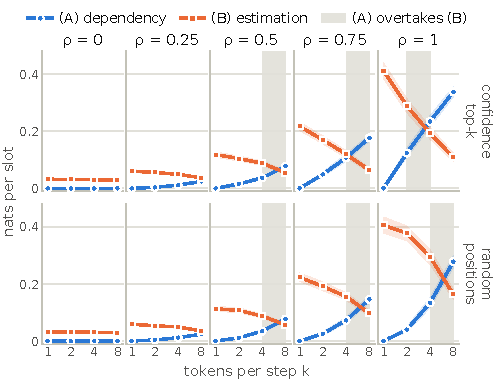
\includegraphics[width=\columnwidth]{artifacts/probe/figures/c2_crossover_ft110m-v3-visible}
  \caption{(A) and (B) per slot (main model), with 95\% intervals, against $k$.
    Columns: $\rho$; rows: selection rule. Shaded: the $k$ where (A) exceeds (B).}
  \label{fig:c2-crossover}
\end{figure}

\subsection{(A) overtakes (B) at high $\rho$ and $k$}
\label{sec:c2-results}

(A) is zero at $k=1$ and at $\rho=0$ and grows with both (Figure~\ref{fig:c2-crossover}).
% Crossover = the first k at which mean (A) > mean (B); none up to k = 8 at rho = 0, 0.25.
% ConfCrossRhoMin = RandCrossRhoMin = 0.5; RandCrossKat{RhoHalf,RhoThreeQuarters,RhoOne} = 8 =
% ConfCrossKat{RhoHalf,RhoThreeQuarters}; CrossKCI* = CrossK* in every main-model cell.
For $\rho\ge\CTwoConfCrossRhoMin$ it overtakes (B) at $k=\CTwoRandCrossKatRhoOne$, or at
$\rho=1$ under confidence top-$k$ already at $k=\CTwoConfCrossKatRhoOne$; each crossover is
also where the 95\% interval of (A)$-$(B) clears zero. For $\rho\le0.25$ (B) dominates up to
$k=8$. At $\rho=1$, $k=8$ (confidence), (A) is \CTwoConfAatRhoOneKEight{}
[\CTwoConfAatRhoOneKEightLo, \CTwoConfAatRhoOneKEightHi] nats per slot and (B)
\CTwoConfBatRhoOneKEight{} [\CTwoConfBatRhoOneKEightLo, \CTwoConfBatRhoOneKEightHi]:
\CTwoConfShareAatRhoOneKEight\% of the total.

% Every cell where ConfB > RandB has overlapping 95% intervals (grid_ft110m-v3-visible.json,
% B_per_field); at rho = 1, k >= 2 ConfB is below RandB.
\paragraph{Confidence selection raises (A), not (B).}
Where (B) is higher under confidence ranking than at random, the intervals overlap. (A) rises instead ($\rho=1$, $k=2$:
\CTwoConfAatRhoOneKTwo{} [\CTwoConfAatRhoOneKTwoLo, \CTwoConfAatRhoOneKTwoHi] against
\CTwoRandAatRhoOneKTwo{} [\CTwoRandAatRhoOneKTwoLo, \CTwoRandAatRhoOneKTwoHi]): the ranking commits
leaders with their followers more often than chance, bringing the crossover forward.

\paragraph{The terms trade off.}
$\rho$ was meant to move only (A), but (B) rises too: at $k=1$, from \CTwoConfBatRhoZeroKOne{}
at $\rho=0$ to \CTwoConfBatRhoOneKOne{} at $\rho=1$. Decoded after its leader, a follower should follow from it, but the model reads the marker
only in part (Appendix~\ref{sec:c2-app}) and stays broad: error in (B). Decoded in the same
step, the true marginal is broad too, and the missing coupling counts as (A). At $\rho=1$, from $k=1$ to $8$, (B) falls to
\CTwoConfBatRhoOneKEight{} while (A) rises from $0$ to \CTwoConfAatRhoOneKEight, so (B)'s fall moves the crossovers too.
% abhiraj, 31 Oct (review): A_per_field means in artifacts/probe/results/grid_ft110m-v3-visible.json vs
%   B_per_field(rho=0, k=1) = 0.032: first k with A > 0.032 is 4 at rho=0.5 and 2 at rho=1 (both rules); none at 0.25.
(A) exceeds the $\rho=0$ (B), \CTwoConfBatRhoZeroKOne{}, from $k=4$ at $\rho=0.5$ and $k=2$ at $\rho=1$. Without
fine-tuning, (B) dominates everywhere ((A) is ${\le}\,$\CTwoUntunedConfShareAMax\% of the
total).

\subsection{Real text: proxies checked on the probe}
\label{sec:c2-text}

The exact values hold for one synthetic distribution and one 110M model; on real text $p^*$
is unknown, so we use proxies. For (A), parallel--sequential disagreement: the fraction of the
$k$ most confident masked positions whose token changes if committed one at a time (earlier
ranks filled with the model's own tokens) instead of in one pass. For (B), the gap
$\Delta=c-a$ and the cross-entropy (CE) of the true token, at the same positions.
% Precisions (110M fp32, LLaDA fp16) are in Table 1 (Sec. 3).
% Mask rates 0.1, 0.2, ..., 1, one state each: config.rates in both T10 JSONs.
We run the 110M model and LLaDA-8B-Base on
\CTwoTTenNDocs{} fit-half FineWeb-Edu documents, one state at each
mask rate $0.1, 0.2, \dots, 1$ (Appendix~\ref{sec:c2-app}), and the proxy on the probe.

\paragraph{The proxy tracks (A) weakly.}
Over the \CTwoTTenProbeNCells{} confidence-rule cells with $k\ge 2$, its Spearman
correlation with the exact (A) is \CTwoTTenProbeSpearman{} [\CTwoTTenProbeSpearmanLo,
\CTwoTTenProbeSpearmanHi]. It rises with $k$,
% 31 Oct (space): the other fine-tune's Spearman, CTwoTTenAltProbeSpearman[Lo|Hi], cut.
barely with $\rho$: at $k=8$, \CTwoTTenProbeDisatRhoZeroKEight{} at $\rho=0$, where (A) is zero,
and \CTwoTTenProbeDisatRhoOneKEight{} at $\rho=1$.

\paragraph{On real text the (A) proxy is near zero.}
% "At most DisKFour at k <= 4": DisKTwo, DisKFour, LladaDisKTwo, LladaDisKFour are all <= DisKFour.
% "Delta cannot be told from zero at k = 1": [DeltaKOneLo, DeltaKOneHi] and the Llada one hold 0.
% "LLaDA does not disagree there": LladaDisKTwo/KFour/KEightRateOne are 0.
Over mask rates 0.1--0.9,
disagreement at $k=8$ is \CTwoTTenDisKEight{} for the 110M model and \CTwoTTenLladaDisKEight{}
for LLaDA, and at most \CTwoTTenDisKFour{} at $k\le4$; at rate 1 (all-\texttt{[MASK]} input), where free generation
starts, it is \CTwoTTenDisKEightRateOne{} for the 110M model and \CTwoTTenLladaDisKEightRateOne{} for LLaDA at $k=8$. CE grows from \CTwoTTenCEKOne{} nats at
$k=1$ to \CTwoTTenCEKEight{} at $k=8$ (LLaDA: \CTwoTTenLladaCEKOne{} to
\CTwoTTenLladaCEKEight), though it includes the text's own entropy and lower ranks are harder
positions. $\Delta$ cannot be told from zero at $k=1$ and is small but positive at $k=8$:
\CTwoTTenDeltaKEight{} [\CTwoTTenDeltaKEightLo, \CTwoTTenDeltaKEightHi] and, for LLaDA,
\CTwoTTenLladaDeltaKEight{} [\CTwoTTenLladaDeltaKEightLo, \CTwoTTenLladaDeltaKEightHi].

So below the all-mask state, committing 2--8 tokens at once rarely changes the models' top
token. The proxy sees only dependence strong enough to flip a top token and barely moves with
$\rho$ on the probe, so this does not show that (A) is small; real text gives a direction, not a split in nats.
